% !TeX program = xelatex
\documentclass[12pt,a4paper]{rapportECL}

% Informations pour la page de garde
\title{GUIDE DE PRÉPARATION INTENSIVE\\CONCOURS DE RECRUTEMENT DES INGÉNIEURS D'ÉTAT (1\textsuperscript{ER} GRADE)\\[0.3cm]\Large MINISTÈRE DE L'ÉCONOMIE ET DES FINANCES}
\author{
    \hspace{0.5cm}$\blacktriangleright$ \textbf{Abdellatif GOURRI}\\[0.1cm]
    \hspace{0.5cm}$\blacktriangleright$ Candidat Ingénieur d'État (1\textsuperscript{er} Grade)\\[0.1cm]
}
\date{\today}
\establishment{\textbf{Royaume du Maroc --- Fonction Publique}}
\department{Ministère de l'Économie et des Finances (MEF)}
\filiere{Préparation Intensive \& Annales d'Épreuves Écrites}

\supervisor{
    \hspace{0.5cm}$\blacktriangleright$ Ministère de l'Économie et des Finances\\[0.1cm]
    \hspace{0.5cm}$\blacktriangleright$ Commission Centrale des Concours
}
\academicyear{\textbf{Session du 20 Septembre 2026}}

\setlength{\parindent}{0pt}
\setlength{\parskip}{0.5em plus 0.2em minus 0.1em}
\linespread{1.15}

\usepackage[french]{babel}
\usepackage{graphicx}
\usepackage{subcaption}
\usepackage{amsmath}
\usepackage{amsfonts}
\usepackage{amssymb}
\usepackage{tikz}
\usepackage{pgfplots}
\pgfplotsset{compat=1.17}
\usepackage[hidelinks]{hyperref}
\usepackage{xurl}

% --- Bibliographie ---
\usepackage[backend=biber,style=ieee]{biblatex}
\addbibresource{references.bib}
\usepackage{needspace}
\usepackage{csquotes}
\usepackage{geometry}
\usepackage{fancyhdr}
\usepackage{setspace}
\usepackage[most]{tcolorbox}
\usepackage{colortbl}
\usepackage{float}
\usepackage{chngcntr}
\usepackage{ltablex}
\usepackage{textcomp}
\usepackage{newunicodechar}
\usepackage{listings}
\usepackage{fontawesome5}
\usepackage{longtable}
\usepackage{array}
\usepackage{booktabs}
\usepackage{enumitem}
\usepackage{tocloft}
\usepackage{multirow}

% =======================================================
% CONFIGURATION TABLE DES MATIERES
% =======================================================
\renewcommand{\thesection}{\arabic{section}-}
\renewcommand{\thesubsection}{\arabic{section} - \arabic{subsection} -}
\renewcommand{\thesubsubsection}{\arabic{section} - \arabic{subsection} - \arabic{subsubsection} -}

\renewcommand{\cftchappresnum}{Chapitre }
\renewcommand{\cftchapaftersnum}{ :}
\setlength{\cftchapnumwidth}{2.4cm}

\renewcommand{\cftchapleader}{\cftdotfill{\cftdotsep}}
\setlength{\cftbeforechapskip}{0.3em}

\setlength{\cftchapindent}{0pt}
\setlength{\cftsecindent}{1.5cm}
\setlength{\cftsecnumwidth}{1.2cm}
\setlength{\cftsubsecindent}{2.5cm}
\setlength{\cftsubsecnumwidth}{2.0cm}

\renewcommand{\cftchapfont}{\normalfont\bfseries}
\renewcommand{\cftchappagefont}{\normalfont\bfseries}
\renewcommand{\cftsecfont}{\normalfont}
\renewcommand{\cftsecpagefont}{\normalfont}
\renewcommand{\cftsubsecfont}{\normalfont}
\renewcommand{\cftsubsecpagefont}{\normalfont}

\renewcommand{\cftfigpresnum}{Figure }
\renewcommand{\cftfigaftersnum}{ :}
\setlength{\cftfignumwidth}{2.8cm}
\renewcommand{\cftfigfont}{\normalfont}
\renewcommand{\cftfigpagefont}{\normalfont}

\renewcommand{\cfttabpresnum}{Tableau }
\renewcommand{\cfttabaftersnum}{ :}
\setlength{\cfttabnumwidth}{3.0cm}
\renewcommand{\cfttabfont}{\normalfont}
\renewcommand{\cfttabpagefont}{\normalfont}

% Normalisation
\newunicodechar{—}{---}
\newunicodechar{–}{--}
\newunicodechar{€}{\texteuro}
\newunicodechar{œ}{\oe}
\newunicodechar{Œ}{\OE}
\newunicodechar{🔴}{\textcolor{red!80!black}{\textbf{\large$\bullet$}}}
\newunicodechar{🟠}{\textcolor{orange!90!black}{\textbf{\large$\bullet$}}}
\newunicodechar{🟡}{\textcolor{yellow!75!black}{\textbf{\large$\bullet$}}}
\newunicodechar{⚪}{\textcolor{gray!60!black}{\textbf{\large$\circ$}}}
\emergencystretch=2em

% Tous les encadrés peuvent se poursuivre sur la page suivante (évite le texte coupé)
\tcbset{breakable}

% Encadré multi-pages pour les dissertations rédigées (copies modèles)
\newtcolorbox{copiemodele}[1]{breakable, enhanced, colback=green!3!white, colframe=green!40!black, fonttitle=\bfseries, title={Copie modèle rédigée --- #1}, before upper={\setlength{\parskip}{0.6em}}}
\newcommand{\partiecopie}[1]{\par\medskip{\color{green!40!black}\textbf{#1}}\par}

\geometry{left=2cm, right=2cm, top=2.5cm, bottom=2.5cm}
\counterwithin{figure}{chapter}
\renewcommand{\thefigure}{\thechapter-\arabic{figure}}
\counterwithin{table}{chapter}
\renewcommand{\thetable}{\thechapter-\arabic{table}}

\renewcommand{\thesection}{\arabic{section} -}
\renewcommand{\thesubsection}{\arabic{section} - \arabic{subsection} -}
\renewcommand{\thesubsubsection}{\arabic{section} - \arabic{subsection} - \arabic{subsubsection} -}

\definecolor{chaporange}{RGB}{15, 60, 110}
\titleformat{\chapter}[block]
  {\normalfont\Large\bfseries\color{chaporange}\centering}
  {\MakeUppercase{\chaptertitlename}~\thechapter~:}
  {1em}
  {\MakeUppercase}

\titleformat{name=\chapter,numberless}[block]
  {\normalfont\Large\bfseries\color{chaporange}\centering}
  {}
  {0pt}
  {\MakeUppercase}

\AtBeginDocument{%
  \setlength{\headheight}{25pt}
  \pagestyle{fancy}
  \fancyhf{}
  \fancyhead[L]{\small\textbf{\textsf{MEF --- Concours Ingénieurs d'État (1\textsuperscript{er} Grade)}}}
  \fancyhead[R]{\small\textbf{\textsf{Préparation Intensive 2026}}}
  \fancyfoot[C]{\thepage}
  \renewcommand{\headrulewidth}{0.5pt}
  \fancypagestyle{plain}{%
    \fancyhf{}
    \fancyhead[L]{\small\textbf{\textsf{MEF --- Concours Ingénieurs d'État (1\textsuperscript{er} Grade)}}}
    \fancyhead[R]{\small\textbf{\textsf{Préparation Intensive 2026}}}
    \fancyfoot[C]{\thepage}
    \renewcommand{\headrulewidth}{0.5pt}%
  }
  \titleformat{\section}{\normalfont\Large\bfseries\color{black}}{\thesection}{1em}{}
  \titleformat{\subsection}[block]{\normalfont\large\bfseries\color{black}\centering}{\thesubsection}{0.8em}{}
  \definecolor{subsubsecblue}{RGB}{31,73,125}
  \titleformat{\subsubsection}{\normalfont\normalsize\itshape\color{subsubsecblue}}{\thesubsubsection}{0.5em}{}
  \renewcommand{\labelitemi}{$\bullet$}
  \renewcommand{\labelitemii}{$\circ$}
}

\begin{document}

\hypersetup{pageanchor=false}
\maketitle
\thispagestyle{empty}
\hypersetup{pageanchor=true}

\newpage
\thispagestyle{empty}
\mbox{}
\newpage

\pagenumbering{Roman}
\setcounter{page}{1}

% --- Résumé Exécutif ---
\chapter*{Résumé Exécutif}
\addcontentsline{toc}{chapter}{Résumé Exécutif}

Le présent document constitue le \textbf{Guide de Préparation Intensive et Haute Rentabilité} destiné aux candidats au concours de recrutement des \textbf{Ingénieurs d'État de 1\textsuperscript{er} grade} du \textbf{Ministère de l'Économie et des Finances (MEF)} du Royaume du Maroc.

Face à la contrainte temporelle extrême (dernière ligne droite avant l'épreuve écrite du \textbf{20 septembre}), l'ensemble des contenus a été sélectionné et structuré selon le principe d'efficacité maximale : \textit{Recherche $\rightarrow$ Vérification $\rightarrow$ Extraction $\rightarrow$ Priorisation $\rightarrow$ Mémorisation ciblée}.

Ce guide s'articule autour de cinq blocs fondamentaux :
\begin{enumerate}[label=\textbf{\arabic*.}]
    \item \textbf{Cadrage et Méthodologie de l'Épreuve Écrite :} Analyse du format de l'examen (sujet de réflexion/dissertation et QCM), grille d'évaluation des correcteurs du MEF, gestion des trois heures, et méthode standardisée de construction de plan en deux parties équilibrées ($I.$ Diagnostic \& Enjeux, $II.$ Stratégies \& Perspectives).
    \item \textbf{Annales Réelles Décortiquées :} Analyse exhaustive des sujets réellement proposés lors des dernières sessions (session du 28 avril 2024 portant sur \textit{Maroc Digital 2030} et la \textit{Transition Énergétique} ; sessions précédentes portant sur \textit{l'Inflation}, le \textit{Déficit Budgétaire}, la \textit{Protection Sociale} et la \textit{Charte de l'Investissement}). Chaque sujet est décomposé selon la formule : \textit{Sujet $\rightarrow$ Problématique $\rightarrow$ Plan détaillé $\rightarrow$ Arguments clés $\rightarrow$ Exemples et chiffres marocains $\rightarrow$ Conclusion}.
    \item \textbf{Banque Exhaustive de Questions / Réponses Normalisée :} Recueil structuré de questions récurrentes issues des annales et concours d'ingénieurs et administrateurs du MEF, classées selon un code de priorité strict (🔴 Très important, 🟠 Important, 🟡 À connaître, ⚪ Secondaire) couvrant l'économie, les finances publiques (LOF 130-13), la modernisation administrative, l'organisation interne du MEF, et les systèmes d'information étatiques.
    \item \textbf{Fiches Mémotechniques « Haute Rentabilité » :} Synthèses condensées sur les missions des directions du MEF (DGI, TGR, Douanes, Budget, DTFE, DEPP, DEPF), les chiffres macroéconomiques clés, les grands principes budgétaires, et les orientations stratégiques du pays.
    \item \textbf{Plan d'Action Sprint Final :} Stratégie de travail par blocs horaires jusqu'au jour de l'examen pour maximiser la rétention et la performance rédactionnelle.
\end{enumerate}


% --- Table des matières ---
\tableofcontents
\newpage

% ---- Liste des sigles et acronymes ----
\chapter*{Liste des Sigles et Acronymes}
\addcontentsline{toc}{chapter}{Liste des Sigles et Acronymes}

\begin{longtable}{p{2.8cm} p{13.5cm}}
\textbf{ADII} & Administration des Douanes et Impôts Indirects \\
\textbf{AMO} & Assurance Maladie Obligatoire \\
\textbf{ANGSPE} & Agence Nationale de Gestion Stratégique des Participations de l'État et de suivi des performances des établissements et entreprises publics \\
\textbf{ASD} & Aide Sociale Directe \\
\textbf{BAM} & Bank Al-Maghrib (Banque centrale du Maroc) \\
\textbf{BGE} & Budget Général de l'État \\
\textbf{BSG} & Budgétisation Sensible au Genre \\
\textbf{CAS} & Compte d'Affectation Spéciale \\
\textbf{CNDP} & Commission Nationale de contrôle de la protection des Données à caractère Personnel \\
\textbf{CST} & Compte Spécial du Trésor \\
\textbf{DAAG} & Direction des Affaires Administratives et Générales \\
\textbf{DB} & Direction du Budget \\
\textbf{DDE} & Direction des Domaines de l'État \\
\textbf{DEPF} & Direction des Études et des Prévisions Financières \\
\textbf{DEPP} & Direction des Entreprises Publiques et de la Privatisation \\
\textbf{DGI} & Direction Générale des Impôts \\
\textbf{DGSSI} & Direction Générale de la Sécurité des Systèmes d'Information \\
\textbf{DNSSI} & Directive Nationale de la Sécurité des Systèmes d'Information \\
\textbf{DTFE} & Direction du Trésor et des Finances Extérieures \\
\textbf{EEP} & Établissements et Entreprises Publics \\
\textbf{GAR} & Gestion Axée sur les Résultats (Gestion par la performance) \\
\textbf{GID} & Gestion Intégrée de la Dépense (Système d'information de la TGR) \\
\textbf{GIR} & Gestion Intégrée des Recettes \\
\textbf{IGF} & Inspection Générale des Finances \\
\textbf{IR} & Impôt sur le Revenu \\
\textbf{IS} & Impôt sur les Sociétés \\
\textbf{LF} & Loi de Finances \\
\textbf{LOF} & Loi Organique n° 130-13 relative à la Loi de Finances \\
\textbf{MEF} & Ministère de l'Économie et des Finances \\
\textbf{NMD} & Nouveau Modèle de Développement \\
\textbf{PIB} & Produit Intérieur Brut \\
\textbf{PLF} & Projet de Loi de Finances \\
\textbf{RNP} & Registre National de la Population \\
\textbf{RSU} & Registre Social Unifié \\
\textbf{SEGMA} & Services de l'État Gérés de Manière Autonome \\
\textbf{SIMPL} & Services des Impôts en Ligne (DGI) \\
\textbf{SI} & Système d'Information \\
\textbf{TGR} & Trésorerie Générale du Royaume \\
\textbf{TVA} & Taxe sur la Valeur Ajoutée \\
\end{longtable}

\newpage

\pagenumbering{arabic}
\setcounter{page}{1}

\chapter*{Introduction Générale}
\addcontentsline{toc}{chapter}{Introduction Générale}

\section*{Le Cadre du Concours de Recrutement}
Le concours d'accès au grade d'\textbf{Ingénieur d'État de premier grade} au sein du \textbf{Ministère des Affaires Étrangères, de la Coopération Africaine et des Marocains Résidant à l'Étranger (MAECAME)} est organisé par la Direction des Affaires Administratives et Générales du ministère, dans le cadre du statut du corps interministériel des ingénieurs et architectes (décret n° 2-05-1367) et du statut particulier du personnel du ministère (décret n° 2-04-534). L'avis de la session 2026 (code C43032/26) ouvre \textbf{16 postes} à l'échelle 11 : \textbf{10 en Réseaux et Télécommunications} et \textbf{6 en Développement informatique}, dont un poste réservé au secteur des Marocains résidant à l'étranger. La sélection est exigeante : \textbf{1 472 candidats} ont été convoqués aux épreuves écrites du 27 septembre 2026, soit environ un poste pour 92 candidats. Lors de la session précédente (23 novembre 2025, 17 postes), environ 943 candidats avaient été convoqués, 149 admis à l'oral et 17 recrutés.

Le ministère n'est pas une administration comme les autres : il porte la voix du Royaume dans le monde, défend son intégrité territoriale, anime sa coopération avec l'Afrique et accompagne plus de cinq millions de Marocains du monde à travers un réseau d'environ 104 ambassades et missions permanentes et 53 consulats généraux répartis sur tous les fuseaux horaires.

\section*{Pourquoi le Ministère recrute-t-il des Ingénieurs d'État ?}
Une diplomatie moderne repose sur des systèmes d'information sûrs, disponibles en permanence et accessibles depuis le monde entier :
\begin{itemize}
    \item \textbf{Réseaux et télécommunications :} interconnexion sécurisée de plus de 150 postes à l'étranger avec l'administration centrale (VPN, liaisons chiffrées, redondance, communications diplomatiques), téléphonie et visioconférence, continuité de service.
    \item \textbf{Services consulaires numériques :} plateformes \texttt{consulat.ma} et \texttt{rdv.consulat.ma}, système interne eConsulat, e-Visa (\texttt{acces-maroc.ma}, lancé en juillet 2022), apostille électronique, état civil consulaire et échanges avec les administrations nationales (Intérieur, Justice, Registre National de la Population).
    \item \textbf{Cybersécurité et protection des données :} le ministère traite des informations sensibles (correspondance diplomatique, données personnelles des Marocains du monde et des demandeurs de visa) soumises à la loi 05-20 sur la cybersécurité, à la Directive Nationale de la Sécurité des Systèmes d'Information (DNSSI) de la DGSSI et à la loi 09-08 sur les données personnelles.
    \item \textbf{Direction des Systèmes d'Information :} créée par le décret n° 2.24.957 du 21 novembre 2024 au sein de la Direction Générale des Affaires Administratives et Générales, elle élabore et exécute les plans du ministère en matière de systèmes d'information, gère l'infrastructure et garantit la cybersécurité.
    \item \textbf{Diplomatie de la donnée et de l'image :} veille et analyse de l'information, communication numérique, tableaux de bord au service de la diplomatie économique et de la mobilisation des compétences des Marocains du monde.
\end{itemize}

\IfFileExists{images/img_001_intro_ecosysteme_si_maecame.png}{%
\begin{figure}[H]
    \centering
    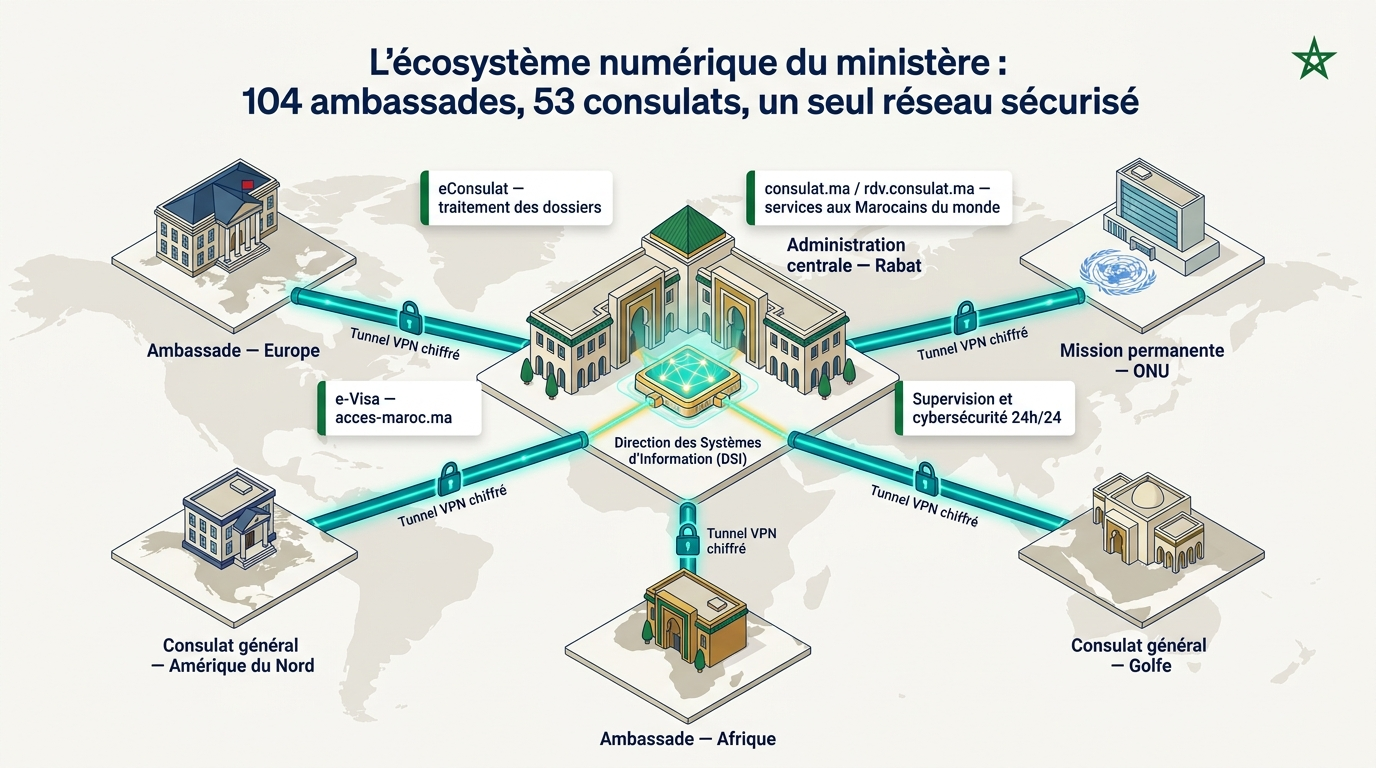
\includegraphics[width=\textwidth]{images/img_001_intro_ecosysteme_si_maecame.png}
    \caption*{\textbf{Illustration introductive :} L'écosystème numérique du MAECAME, de l'administration centrale au réseau diplomatique et consulaire}
\end{figure}}{}

Le jury attend donc un \textbf{ingénieur solide techniquement} (l'épreuve de spécialité compte pour un tiers de la note finale, et l'oral, largement technique, pour la moitié), mais aussi un \textbf{cadre de l'État capable de comprendre les missions du ministère} et d'inscrire ses solutions dans les priorités de la diplomatie marocaine.

\section*{Les Trois Épreuves et leur Poids}
\begin{table}[H]
\centering
\small
\begin{tabular}{|p{5.2cm}|c|c|c|p{4.6cm}|}
\hline
\rowcolor{gray!20} \textbf{Épreuve} & \textbf{Durée} & \textbf{Coef.} & \textbf{Poids} & \textbf{Contenu (avis officiel)} \\ \hline
Écrit (a) : Spécialité & 3 h & 4 & 33 \% & Spécialité(s) demandée(s), fonctions ou postes à occuper en informatique et en réseaux. \\ \hline
Écrit (b) : Rédaction & 2 h & 2 & 17 \% & Rédaction d'un sujet portant sur les attributions du ministère. \\ \hline
Oral : Entretien & 30-40 min & 6 & 50 \% & Discussion avec le jury de sujets et questions variés pour évaluer l'aptitude à exercer les fonctions. \\ \hline
\end{tabular}
\caption{Barème du concours 2026 (avis officiel C43032/26)}
\end{table}

\IfFileExists{images/img_011_bareme_trois_epreuves.png}{%
\begin{figure}[H]
    \centering
    
\includegraphics[width=\textwidth]{images/img_011_bareme_trois_epreuves.png}
    \caption*{Le barème du concours : où concentrer l'effort}
\end{figure}}{}

L'avis ne précise ni la forme exacte de l'épreuve de spécialité (QCM, questions ouvertes ou exercices), ni la langue, ni un seuil d'admissibilité : il faut se préparer à toutes les formes et savoir rédiger en français comme en arabe pour les notions institutionnelles.

\section*{Objectif et Organisation du Présent Guide}
Face à une échéance à quatre jours, ce guide vise l'efficacité immédiate :
\begin{enumerate}
    \item \textbf{Comprendre ce qui est réellement noté :} les trois épreuves, leur poids et les attentes d'un jury de diplomates et d'ingénieurs.
    \item \textbf{Maîtriser la matière diplomatique :} organisation du ministère, constantes de la politique étrangère, Sahara, Afrique, Marocains du monde, partenariats, avec des sujets de rédaction entièrement traités.
    \item \textbf{Réussir l'épreuve de spécialité :} réseaux et télécommunications, développement et bases de données, cybersécurité, avec exercices corrigés adaptés au contexte du ministère.
    \item \textbf{S'entraîner en conditions réelles :} planning J-4 et examen blanc complet avec corrigés.
\end{enumerate}


% --- PREMIÈRE PARTIE : MÉTHODOLOGIE ET ANNALES DE DISSERTATION ---
\part{MÉTHODOLOGIE ET ANNALES DE DISSERTATION}

\chapter{Structure de l'Épreuve Écrite et Méthodologie de Réussite}

\section{Format et Modalités de l'Épreuve Écrite}
Les concours de recrutement des Ingénieurs d'État (1\textsuperscript{er} grade) au sein du Ministère de l'Économie et des Finances se caractérisent généralement par une épreuve écrite d'une durée de \textbf{3 heures} (coefficient 4 ou selon l'avis de concours), suivie pour les admissibles d'un entretien oral (coefficient 3).

L'épreuve écrite se présente selon l'une des deux configurations majeures adoptées par le ministère ces dernières années :
\begin{enumerate}
    \item \textbf{Configuration A (Format Prédominant - Sujet de Réflexion / Dissertation Générale \& Économique) :}
    Deux sujets d'actualité stratégique, économique, numérique ou financière sont proposés au choix du candidat, à rédiger en français ou en arabe (ex. session du 28 avril 2024 : Sujet 1 sur la digitalisation / \textit{Maroc Digital 2030}, Sujet 2 sur la transition et sécurité énergétique).
    \item \textbf{Configuration B (Format Hybride - Dissertation + QCM / Questions à Réponses Courtes) :}
    Une partie de culture générale financière, administrative et institutionnelle sous forme de QCM (missions du MEF, Loi Organique de Finances 130-13, finances publiques, fiscalité, déontologie administrative), complétée par une question rédactionnelle d'analyse ou de synthèse technique.
\end{enumerate}

\section{Grille de Notation et Attentes Réelles des Correcteurs du MEF}
Les correcteurs sont des hauts fonctionnaires, directeurs ou inspecteurs du MEF, ainsi que des universitaires. Leurs critères d'appréciation s'articulent autour de cinq axes majeurs :
\begin{table}[H]
\centering
\small
\begin{tabular}{|p{4.5cm}|c|p{8.5cm}|}
\hline
\rowcolor{gray!20} \textbf{Critère d'évaluation} & \textbf{Pondération} & \textbf{Ce que recherche le jury} \\ \hline
\textbf{Structure et Logique du Plan} & 25\% & Problématique claire, plan en deux parties équilibrées (I et II) avec sous-parties (A et B), transitions soignées, respect de la démarche déductive. \\ \hline
\textbf{Maîtrise du Contexte Marocain} & 30\% & Connaissance précise des stratégies nationales (\textit{Maroc Digital 2030}, Charte de l'Investissement, LOF 130-13), citations de lois, chiffres récents, références institutionnelles. \\ \hline
\textbf{Vision de l'Ingénieur d'État} & 20\% & Capacité à lier les enjeux technologiques/techniques à l'efficacité économique, à la rationalisation des coûts et à l'impact citoyen. \\ \hline
\textbf{Qualité Rédactionnelle et Clarté} & 15\% & Style administratif rigoureux, vocabulaire économique précis, orthographe et syntaxe irréprochables, présentation aérée. \\ \hline
\textbf{Esprit Critique et Propositions} & 10\% & Diagnostic lucide des défis et formulation de recommandations réalistes et constructives pour l'administration. \\ \hline
\end{tabular}
\caption{Grille type d'évaluation des épreuves écrites du MEF}
\end{table}

\section{Gestion Optimale du Temps sur 3 Heures (180 Minutes)}
La principale cause d'échec n'est pas le manque de connaissances, mais le manque de temps à la fin de l'épreuve. Voici le découpage chronométré à appliquer rigoureusement :
\begin{itemize}
    \item \textbf{00h00 - 00h15 (15 min) : Choix du sujet et Définition des termes clés}
    Lire attentivement les deux sujets. Choisir celui où l'on dispose du plus grand nombre d'exemples et de chiffres marocains précis. Définir chaque mot du sujet pour éviter le hors-sujet.
    \item \textbf{00h15 - 00h45 (30 min) : Brainstorming, Problématique et Élaboration du Plan détaillé}
    Jeter les idées au brouillon, les classer, formuler la problématique centrale sous forme de question directrice, et construire le plan :
    \begin{center}
    \textbf{I. Diagnostic, État des lieux et Enjeux} (A. Réalisations / B. Limites \& Défis) \\
    \textbf{II. Orientations Stratégiques, Leviers Opérationnels et Perspectives} (A. Cadre stratégique / B. Recommandations)
    \end{center}
    \item \textbf{00h45 - 01h00 (15 min) : Rédaction intégrale de l'Introduction et de la Conclusion au brouillon}
    C'est la première et la dernière impression laissée au correcteur. Elles doivent être parfaites.
    \item \textbf{01h00 - 02h45 (1h45) : Rédaction directe sur la copie d'examen}
    Rédiger directement le corps du texte (Parties I et II) en s'appuyant sur le plan détaillé du brouillon. Soigner les chapeaux introductifs et les phrases de transition.
    \item \textbf{02h45 - 03h00 (15 min) : Relecture impérative}
    Chasse aux fautes d'accord, de ponctuation, vérification de la lisibilité des titres et des chiffres.
\end{itemize}

\section{La Méthode Infaillible de la Dissertation Administrative}

\subsection{L'Introduction en 5 Étapes Indispensables}
Une introduction réussie doit comporter obligatoirement les 5 étapes suivantes en un ou deux paragraphes cohérents :
\begin{enumerate}
    \item \textbf{L'Accroche (Amorce) :} Partir d'une dynamique générale contemporaine, d'un discours royal, d'un événement économique majeur ou d'une mutation globale.
    \item \textbf{Définition et Cadrage du Sujet :} Définir les concepts centraux (ex. digitalisation, transition énergétique, souveraineté économique).
    \item \textbf{Contexte Marocain :} Présenter la place de cette thématique dans les politiques publiques nationales (réformes du MEF, Nouveau Modèle de Développement, Lois de Finances).
    \item \textbf{La Problématique :} Poser la question de fond qui structure toute la réflexion.
    \item \textbf{L'Annonce du Plan :} Annoncer explicitement et élégamment les deux parties principales.
\end{enumerate}

\subsection{La Règle d'Or du Plan en Deux Parties}
La tradition des concours de la fonction publique marocaine et des grands corps d'ingénieurs privilégie le plan binaire équilibré :
\begin{itemize}
    \item \textbf{Partie I : État des Lieux, Acquis et Diagnostic Critique}
    \begin{itemize}
        \item \textit{Sous-partie I.A :} Les réalisations majeures, le cadre institutionnel et les progrès enregistrés au Maroc.
        \item \textit{Sous-partie I.B :} Les contraintes structurelles, les insuffisances et les défis persistants.
    \end{itemize}
    \item \textbf{Partie II : Stratégies Nationales, Rôle de l'Ingénieur et Leviers d'Avenir}
    \begin{itemize}
        \item \textit{Sous-partie II.A :} Les programmes et feuilles de route gouvernementales (ex. stratégies sectorielles, lois-cadres).
        \item \textit{Sous-partie II.B :} Recommandations opérationnelles, modernisation des processus, gouvernance et perspectives d'impact.
    \end{itemize}
\end{itemize}

\subsection{La Conclusion Efficace}
La conclusion doit comprendre deux volets :
\begin{enumerate}
    \item \textbf{Le Bilan (Synthèse) :} Répondre synthétiquement à la problématique sans répéter le texte.
    \item \textbf{L'Ouverture :} Élargir sur un enjeu complémentaire (ex. intégration régionale africaine, souveraineté industrielle, impact de l'intelligence artificielle générative).
\end{enumerate}

\chapter{Annales Réelles et Décorticage des Sujets de Dissertation}

Ce chapitre présente l'analyse approfondie des sujets \textbf{réellement posés} lors des récentes sessions du concours d'Ingénieurs d'État du Ministère de l'Économie et des Finances, ainsi que les sujets à très haute probabilité issus des réformes majeures de l'État.

Chaque sujet est traité selon la matrice exigée :
\begin{center}
\textbf{Sujet $\longrightarrow$ Problématique $\longrightarrow$ Plan détaillé $\longrightarrow$ Idées principales $\longrightarrow$ Exemples marocains $\longrightarrow$ Conclusion}
\end{center}

% =========================================================================
\section{Sujet 1 (Session Réelle du 28 Avril 2024) : Digitalisation et Stratégie « Maroc Digital 2030 »}
% =========================================================================

\begin{tcolorbox}[colback=blue!5!white,colframe=blue!75!black,title=\textbf{Énoncé Officiel du Sujet (28 Avril 2024)}]
\textit{« Durant les dernières années, le Maroc a fait beaucoup de réalisations dans le domaine de la digitalisation. Quel bilan faites-vous de ces réalisations ? Quelles sont les axes prioritaires de la Stratégie Maroc Digital 2030 et les orientations stratégiques pour accompagner cette transition ? »}
\end{tcolorbox}

\subsection*{1. Problématique}
Dans quelle mesure les acquis de la transition numérique marocaine constituent-ils un levier de modernisation économique et administrative, et comment la stratégie « Maroc Digital 2030 » entend-elle surmonter les fractures structurelles pour faire du digital un vecteur de souveraineté et d'inclusion ?

\subsection*{2. Plan Détaillé Proposé}
\begin{itemize}
    \item \textbf{I. Le Bilan de la Digitalisation au Maroc : Des Avancées Notables Face à des Freins Persistants}
    \begin{itemize}
        \item \textbf{A.} Des réalisations substantielles dans les services publics et l'offshoring.
        \item \textbf{B.} Des limites structurelles : fracture territoriale, compétences et inclusion des TPME.
    \end{itemize}
    \item \textbf{II. La Stratégie « Maroc Digital 2030 » et les Leviers d'Accompagnement de la Transition}
    \begin{itemize}
        \item \textbf{A.} Les deux piliers et catalyseurs prioritaires de la feuille de route 2030.
        \item \textbf{B.} Les orientations stratégiques d'accompagnement : souveraineté des données, 5G, talents et gouvernance.
    \end{itemize}
\end{itemize}

\subsection*{3. Idées Principales et Arguments}
\begin{itemize}
    \item \textbf{Pour le bilan (Partie I) :}
    \begin{itemize}
        \item Émergence du Maroc comme 2\textsuperscript{e} hub d'outsourcing en Afrique (plus de 130 000 emplois créés, exportations de services IT en forte croissance).
        \item Révolution des services publics dématérialisés : téléprocédures fiscales (SIMPL de la DGI), douanières (BADR de l'ADII), marchés publics électroniques (TGR), et simplification administrative (Loi 55-19 et portail national \textit{Idarati}).
        \item Limites : persistance de la fracture numérique entre zones urbaines et rurales, taux d'adoption digital encore faible chez les TPME traditionnelles, déficit en compétences pointues (fuite des cerveaux IT), et manque d'interopérabilité fluide entre ministères.
    \end{itemize}
    \item \textbf{Pour Maroc Digital 2030 (Partie II) :}
    \begin{itemize}
        \item \textbf{Pilier 1 : Digitalisation des services publics} (atteindre un parcours 100\% digitalisé et ergonomique, guichet unique, interopérabilité généralisée).
        \item \textbf{Pilier 2 : Dynamisation de l'économie numérique} (développer les startups, exporter des solutions numériques locales, attirer les investissements étrangers dans la tech).
        \item \textbf{Catalyseurs clés :} Déploiement de la 5G, développement d'un Cloud souverain national, formation de 100 000 jeunes talents par an d'ici 2030, intégration de l'Intelligence Artificielle dans l'analyse de données fiscales et financières.
    \end{itemize}
\end{itemize}

\subsection*{4. Exemples et Données Marocaines Précises}
\begin{itemize}
    \item Budget alloué à la première phase (2024-2026) : environ 11 milliards de dirhams.
    \item Cadre juridique : Loi n° 09-08 (protection des données personnelles via la CNDP), Loi n° 43-20 (services de confiance pour les transactions électroniques), et Loi n° 55-19 (simplification des procédures administratives).
    \item Direction Générale de la Sécurité des Systèmes d'Information (DGSSI) et Directive Nationale de la Sécurité des SI (DNSSI).
    \item Écosystème startups : Fonds InnovX, programmes de la Caisse des Dépôts et de Gestion (CDG Invest).
\end{itemize}

\subsection*{5. Conclusion et Ouverture}
Le Maroc passe d'une numérisation d'appoint à une véritable économie de la donnée. L'enjeu futur réside dans la souveraineté numérique (Data Centers locaux) et l'utilisation de l'intelligence artificielle pour optimiser les recettes fiscales et lutter contre l'économie informelle.

% =========================================================================
\section{Sujet 2 (Session Réelle du 28 Avril 2024) : Transition et Sécurité Énergétique au Maroc}
% =========================================================================

\begin{tcolorbox}[colback=blue!5!white,colframe=blue!75!black,title=\textbf{Énoncé Officiel du Sujet (28 Avril 2024)}]
\textit{« À l'aune de la crise énergétique que traverse l'économie mondiale, l'accélération de la transition énergétique est placée au centre des priorités du développement économique de notre pays. Quels sont les nouveaux enjeux de la sécurité énergétique au Maroc ? Quels sont les axes stratégiques pour renforcer cette sécurité et les défis liés à la stratégie nationale de transition énergétique ? »}
\end{tcolorbox}

\subsection*{1. Problématique}
Face aux chocs géopolitiques et à la volatilité des marchés énergétiques internationaux, comment le Maroc peut-il concilier l'impératif immédiat de sécurisation de ses approvisionnements avec l'ambition durable d'une transition énergétique basée sur les énergies renouvelables et l'hydrogène vert ?

\subsection*{2. Plan Détaillé Proposé}
\begin{itemize}
    \item \textbf{I. Les Nouveaux Enjeux de la Sécurité Énergétique Marocaine : Vulnérabilités et Défis}
    \begin{itemize}
        \item \textbf{A.} La dépendance énergétique externe et l'impact direct sur les finances publiques.
        \item \textbf{B.} L'impératif de décarbonation industrielle et les nouvelles exigences climatiques mondiales.
    \end{itemize}
    \item \textbf{II. Les Axes Stratégiques et les Leviers Opérationnels de la Transition Énergétique}
    \begin{itemize}
        \item \textbf{A.} L'accélération du mix renouvelable et le déploiement de « l'Offre Maroc » pour l'Hydrogène Vert.
        \item \textbf{B.} Efficacité énergétique, interconnexions régionales et défis de financement.
    \end{itemize}
\end{itemize}

\subsection*{3. Idées Principales et Données Marocaines}
\begin{itemize}
    \item Taux de dépendance énergétique du Maroc : passé de plus de 98\% au début des années 2000 à environ 90\% aujourd'hui, avec un coût lourd sur la balance commerciale et les charges de compensation.
    \item Objectif national fixé par les Orientations Royales : dépasser 52\% de capacité électrique installée d'origine renouvelable (solaire, éolien, hydraulique) avant 2030.
    \item Réalisations majeures : Complexe solaire Noor Ouarzazate (580 MW), parcs éoliens de Tarfaya et Midelt, stations de transfert d'énergie par pompage (STEP Abdelmoumen).
    \item « Offre Maroc » pour l'hydrogène vert (circulaire du Chef du Gouvernement de mars 2024) : mobilisation de 1 million d'hectares de foncier public pour attirer les investisseurs mondiaux.
    \item Rôle du MEF : financement vert, partenariats public-privé (loi 86-12), et décarbonation pour anticiper le Mécanisme d'Ajustement Carbone aux Frontières (MACF) de l'Union Européenne.
\end{itemize}

\subsection*{4. Conclusion}
La transition énergétique marocaine n'est plus seulement un choix écologique, mais une exigence de compétitivité industrielle et de souveraineté budgétaire.

% =========================================================================
\section{Sujet 3 (Sessions Réelles 2022-2023) : L'Inflation et la Préservation du Pouvoir d'Achat}
% =========================================================================

\begin{tcolorbox}[colback=blue!5!white,colframe=blue!75!black,title=\textbf{Énoncé Réel / Thème Fréquent}]
\textit{« L'inflation au Maroc s'est nettement accélérée ces dernières années. Quelles sont les principales causes de cette hausse continue des prix ? Quelles sont ses répercussions économiques et sociales et quelles sont les mesures de politique économique et budgétaire adoptées ou recommandées pour y faire face ? »}
\end{tcolorbox}

\subsection*{1. Problématique}
Quelles sont les dynamiques internes et externes expliquant la flambée inflationniste récente au Maroc, et quelle articulation entre politique monétaire (Bank Al-Maghrib) et politique budgétaire (MEF) permet de contenir la hausse des prix sans étouffer la croissance ?

\subsection*{2. Plan Détaillé}
\begin{itemize}
    \item \textbf{I. Diagnostic de l'Inflation : Causes Multiples et Impacts Socio-Économiques}
    \begin{itemize}
        \item \textbf{A.} Les facteurs déclencheurs : inflation importée (énergie, matières premières) et facteurs climatiques (sécheresse sévère affectant les prix agricoles).
        \item \textbf{B.} Les conséquences : érosion du pouvoir d'achat des ménages, hausse des coûts de production et tension sur le budget de l'État.
    \end{itemize}
    \item \textbf{II. Les Réponses des Politiques Publiques et les Perspectives de Stabilisation}
    \begin{itemize}
        \item \textbf{A.} La politique monétaire de Bank Al-Maghrib : relèvements successifs du taux directeur.
        \item \textbf{B.} Les mesures budgétaires du MEF et réformes structurelles : soutien aux intrants agricoles, subventions ciblées et réorganisation des circuits de commercialisation.
    \end{itemize}
\end{itemize}

\subsection*{3. Chiffres et Faits Marocains Clés}
\begin{itemize}
    \item Pic d'inflation en 2022-2023 (6,6\% en 2022, 6,1\% en 2023), tirée principalement par les produits alimentaires (+15\% à son pic), avant une décélération progressive en 2024 vers 1,5\% à 2\%.
    \item Décisions de Bank Al-Maghrib : augmentation graduelle du taux directeur de 1,50\% jusqu'à 3,00\% pour freiner les anticipations inflationnistes, puis premier assouplissement à 2,75\% en juin 2024 face à l'accalmie des prix.
    \item Mesures MEF : soutien direct aux professionnels du transport routier pour éviter la répercussion sur les prix à la consommation, suspension des droits de douane et de la TVA sur l'importation de bétail et d'huile, et enveloppes exceptionnelles de la Caisse de Compensation (gaz butane, blé, sucre).
\end{itemize}

% =========================================================================
\section{Sujet 4 (Session Réelle 2021-2022) : Maîtrise du Déficit Budgétaire et Dette Publique}
% =========================================================================

\begin{tcolorbox}[colback=blue!5!white,colframe=blue!75!black,title=\textbf{Énoncé Réel}]
\textit{« Le déficit des finances publiques constitue une caractéristique structurelle de l'économie marocaine. Quelles sont, à votre avis, les mesures à adopter pour maîtriser l'impact de ce déficit tout en préservant la dynamique d'investissement et les impératifs sociaux ? »}
\end{tcolorbox}

\subsection*{1. Problématique}
Comment l'État marocain peut-il réussir l'équation complexe de la consolidation budgétaire (réduction du déficit sous 4\% du PIB) tout en finançant les chantiers stratégiques de l'État social et les grands investissements d'infrastructures ?

\subsection*{2. Plan Détaillé}
\begin{itemize}
    \item \textbf{I. La Problématique du Déficit Budgétaire et de la Dette : Facteurs et Contraintes}
    \begin{itemize}
        \item \textbf{A.} Les causes structurelles du déficit : rigidité des dépenses obligatoires (masse salariale, charge de la dette, compensation).
        \item \textbf{B.} Le risque d'éviction et les seuils d'alerte de l'endettement du Trésor ($\approx 70\%$ du PIB).
    \end{itemize}
    \item \textbf{II. La Stratégie d'Assainissement Budgétaire et les Nouveaux Leviers de Financement}
    \begin{itemize}
        \item \textbf{A.} L'élargissement de l'assiette fiscale et la rationalisation des dépenses (LOF 130-13 et Loi-cadre 69-19).
        \item \textbf{B.} Les mécanismes innovants de financement et le partenariat public-privé (Fonds Mohammed VI pour l'Investissement, ANGSPE).
    \end{itemize}
\end{itemize}

\subsection*{3. Chiffres et Références Institutionnelles}
\begin{itemize}
    \item Évolution du déficit budgétaire : de plus de 7\% du PIB en 2020 (crise Covid) à 4,3\% en 2023, avec pour cible 4\% en 2024 et 3,5\% à l'horizon 2025-2026.
    \item Dette du Trésor : stabilisée autour de 69,5\% à 70\% du PIB, avec une composante intérieure prédominante (environ 75\% de la dette) limitant le risque de change.
    \item Financements innovants : monétisation d'actifs immobiliers de l'État par la Direction des Domaines et gestion active du portefeuille d'entreprises publiques.
\end{itemize}

% =========================================================================
\section{Sujet 5 (Thème Royal Majeur) : Généralisation de la Protection Sociale}
% =========================================================================

\begin{tcolorbox}[colback=blue!5!white,colframe=blue!75!black,title=\textbf{Thème Stratégique et Sujet Très Probable}]
\textit{« Le chantier de la généralisation de la protection sociale au Maroc : réalisations, modalités de financement, soutenabilité budgétaire et défis de mise en œuvre. »}
\end{tcolorbox}

\subsection*{1. Problématique}
En quoi la généralisation de la protection sociale représente-t-elle un changement de paradigme vers un véritable État social, et quelles sont les conditions de sa pérennité budgétaire et opérationnelle ?

\subsection*{2. Plan Détaillé}
\begin{itemize}
    \item \textbf{I. Un Projet Sociétal d'Envergure : Piliers et Réalisations Concrètes}
    \begin{itemize}
        \item \textbf{A.} La feuille de route de la Loi-cadre 09-21 : de l'AMO de base à l'Aide Sociale Directe (ASD).
        \item \textbf{B.} Le rôle pivot des outils de ciblage : Registre National de la Population (RNP) et Registre Social Unifié (RSU).
    \end{itemize}
    \item \textbf{II. Le Défi Majeur de la Soutenabilité Budgétaire et de l'Efficience Opérationnelle}
    \begin{itemize}
        \item \textbf{A.} Les mécanismes de financement : articulation entre cotisations contributives et solidarité budgétaire de l'État.
        \item \textbf{B.} Les réformes indispensables d'accompagnement : refonte du système national de santé et réforme de la Caisse de Compensation.
    \end{itemize}
\end{itemize}

\subsection*{3. Données Clés}
\begin{itemize}
    \item Coût global annuel du chantier : environ 51 milliards de dirhams par an, dont près de 25 milliards financés directement par le budget de l'État.
    \item Calendrier : AMO pour tous fin 2022 (transition du RAMED vers AMO Tadamon), lancement des aides directes fin 2023 (allocations de 500 à 1000 DH/mois par famille ciblée), extension prévue pour les régimes de retraite et l'indemnité pour perte d'emploi.
\end{itemize}


% --- DEUXIÈME PARTIE : BANQUE DE QUESTIONS ET FICHES RÉVISIONS ---
\part{BANQUE DE QUESTIONS / RÉPONSES ET FICHES MÉMOTECHNIQUES}

\chapter{Banque de Questions / Réponses et Préparation de l'Épreuve de Spécialité}

Ce chapitre comprend deux volets : (1) une banque de questions/réponses sur le \textbf{ministère et la politique étrangère}, utile pour la rédaction et surtout pour l'oral (coefficient 6) ; (2) la préparation de l'\textbf{épreuve écrite de spécialité} (3 heures, coefficient 4) en informatique et réseaux, avec des questions/réponses par thème et des \textbf{exercices rédigés corrigés} placés dans le contexte du ministère.

\section*{Légende des Niveaux de Priorité et de Typologie}
\begin{itemize}
    \item \textbf{Priorité :}
    \textbf{🔴 Très important} (attribution centrale du ministère ou actualité majeure) ;
    \textbf{🟠 Important} (notion institutionnelle ou diplomatique fondamentale) ;
    \textbf{🟡 À connaître} (notion utile) ;
    \textbf{⚪ Secondaire} (culture générale).
    \item \textbf{Type :}
    \textbf{[Officiel]} = tiré de l'avis de concours ou d'un texte officiel ;
    \textbf{[Actualité]} = fait daté de 2024-2026 ;
    \textbf{[Thème récurrent]} = question classique des jurys de la fonction publique ;
    \textbf{[Prépa]} = question conçue pour ce guide.
\end{itemize}

\section{Volet 1 : Ministère, Diplomatie et Marocains du Monde}

{\footnotesize
\setlength{\tabcolsep}{3pt}
\begin{longtable}{|>{\raggedright\arraybackslash\hspace{0pt}}p{3.9cm}|>{\raggedright\arraybackslash\hspace{0pt}}p{5.1cm}|>{\raggedright\arraybackslash\hspace{0pt}}p{2.1cm}|>{\raggedright\arraybackslash\hspace{0pt}}p{2.3cm}|>{\raggedright\arraybackslash\hspace{0pt}}p{1.5cm}|c|}
\hline
\rowcolor{gray!20} \textbf{Question} & \textbf{Réponse Synthétique} & \textbf{Thème} & \textbf{Source} & \textbf{Type} & \textbf{Prio} \\ \hline
\endfirsthead
\hline
\rowcolor{gray!20} \textbf{Question} & \textbf{Réponse Synthétique} & \textbf{Thème} & \textbf{Source} & \textbf{Type} & \textbf{Prio} \\ \hline
\endhead

Quelles sont les trois épreuves du concours d'ingénieurs d'État du MAECAME 2026 ? & Écrit de spécialité informatique et réseaux (3 h, coef. 4) ; rédaction d'un sujet sur les attributions du ministère (2 h, coef. 2) ; entretien oral (30-40 min, coef. 6). & Concours & Avis C43032/26 & [Officiel] & 🔴 \\ \hline

Combien de postes sont ouverts et dans quelles spécialités ? & 16 postes (échelle 11) : 10 en Réseaux et Télécommunications, 6 en Développement informatique, dont 1 poste dédié au secteur des MRE. & Concours & Avis C43032/26 & [Officiel] & 🔴 \\ \hline

Quelles sont les grandes attributions du ministère ? & Conduire la politique étrangère sous l'autorité du Roi (intégrité territoriale, bilatéral, multilatéral) ; coopération africaine et Sud-Sud ; service et protection des MRE ; diplomatie économique et culturelle ; gestion du réseau diplomatique et consulaire. & Ministère & Décret 2.24.957 & [Officiel] & 🔴 \\ \hline

Qui est le ministre des Affaires étrangères et depuis quand ? & M. Nasser Bourita, depuis le 5 avril 2017, reconduit le 23 octobre 2024 ; gouvernement sortant après les législatives du 23 septembre 2026. & Ministère & Presse officielle & [Actualité] & 🔴 \\ \hline

Quel texte a réorganisé le ministère en 2024 et qu'a-t-il changé ? & Le décret n° 2.24.957 du 21 novembre 2024 : regroupement en pôles, nouvelles directions (dont la Direction des Systèmes d'Information au sein de la DGAAG), transformation de l'AMED en IMFRED. & Ministère & BO / presse & [Officiel] & 🔴 \\ \hline

Quelle est la mission de la Direction des Systèmes d'Information du ministère ? & Élaborer et exécuter les plans du ministère en matière de SI, gérer l'infrastructure et garantir la cybersécurité, pour l'administration centrale et le réseau à l'étranger. & Ministère / SI & Décret 2.24.957 & [Officiel] & 🔴 \\ \hline

Quelle est la taille du réseau diplomatique et consulaire ? & Environ 104 ambassades et missions permanentes et 53 consulats généraux ; 21 nouveaux consuls généraux nommés en 2026 (35 \% des postes). & Ministère & Presse 2026 & [Actualité] & 🟠 \\ \hline

Qu'est-ce que la DACS ? & La Direction des Affaires Consulaires et Sociales : état civil, documents, protection et assistance des Marocains à l'étranger, statistiques consulaires. & Ministère & Organigramme & [Thème récurrent] & 🟠 \\ \hline

Qu'est-ce que l'AMCI ? & L'Agence Marocaine de Coopération Internationale (1986), bras de la coopération Sud-Sud : bourses d'étudiants étrangers (surtout africains), formation, expertise. & Coopération & AMCI & [Thème récurrent] & 🟠 \\ \hline

Qu'est-ce que l'IMFRED ? & L'Institut Marocain de Formation, de Recherche et d'Études Diplomatiques, qui remplace l'Académie Marocaine des Études Diplomatiques (2011) ; forme les diplomates. & Ministère & Décret 2.24.957 & [Officiel] & 🟡 \\ \hline

Quels articles de la Constitution concernent les MRE ? & Articles 16 (protection des droits et intérêts), 17 (droits de citoyenneté, vote), 18 (participation aux institutions consultatives) ; article 163 (CCME). & MRE & Constitution 2011 & [Thème récurrent] & 🔴 \\ \hline

Quelles institutions s'occupent des MRE et que change la réforme de 2024 ? & Ministère (DACS, consulats), CCME (2007), Fondation Hassan II (1990), Fondation Mohammed V (Marhaba). Discours du 6 novembre 2024 : CCME recentré sur la prospective, création d'une Fondation Mohammedia des MRE (bras opérationnel) et d'un mécanisme de mobilisation des compétences ; textes en cours. & MRE & Discours royal 2024 & [Actualité] & 🔴 \\ \hline

Chiffres clés des MRE ? & Plus de 5 millions de personnes ; transferts 117,7 MMDH en 2024 (7,7 \% du PIB), plus de 122 MMDH en 2025, 74,78 MMDH à fin juillet 2026 ; Marhaba 2026 : 4,14 millions accueillis. & MRE & Office des changes / FM5 & [Actualité] & 🔴 \\ \hline

Comment les MRE ont-ils voté aux législatives de 2026 ? & Par procuration, via une plateforme dématérialisée « E-procuration » (24 août -- 22 septembre 2026) ; pas de bureaux de vote à l'étranger. & MRE & FH2MRE & [Actualité] & 🟡 \\ \hline

Que dit la résolution 2797 du Conseil de sécurité ? & Adoptée le 31 octobre 2025 (11 pour, 3 abstentions, l'Algérie ne participant pas) : l'autonomie sous souveraineté marocaine est la base des négociations et « la solution la plus réalisable » ; MINURSO prorogée jusqu'au 31 octobre 2026. & Sahara & ONU & [Actualité] & 🔴 \\ \hline

Quels pays ou organisations soutiennent explicitement le plan d'autonomie ? & États-Unis (10 déc. 2020, réaffirmé avril 2025), Espagne (mars 2022), France (30 juillet 2024), Royaume-Uni (1\textsuperscript{er} juin 2025), Union européenne (position commune du 29 janvier 2026), et une large majorité d'États arabes et africains ; une trentaine de consulats à Laâyoune et Dakhla. & Sahara & Fiche 3 & [Actualité] & 🔴 \\ \hline

Quels sont les six principes énoncés par le Maroc à l'ONU le 22 septembre 2026 ? & Pas de solution hors autonomie sous souveraineté marocaine ; négociation onusienne sur la seule base de l'Initiative ; obligations de la 2797 non négociables ; refus du statu quo ; crédibilité liée au respect du cessez-le-feu ; libération des populations de Tindouf. & Sahara & AGNU 2026 & [Actualité] & 🔴 \\ \hline

Quand le Maroc est-il revenu à l'Union Africaine et pourquoi l'avait-il quittée ? & Retour le 30 janvier 2017 ; retrait de l'OUA en 1984 après l'admission de la « RASD ». Demande d'adhésion à la CEDEAO en 2017, toujours en attente. & Afrique & UA & [Thème récurrent] & 🔴 \\ \hline

Qu'est-ce que l'Initiative Atlantique ? & Initiative royale de novembre 2023 offrant aux pays du Sahel (Mali, Burkina Faso, Niger, Tchad) un accès à l'Atlantique via les infrastructures marocaines, notamment le port Dakhla Atlantique. & Afrique & Discours royal & [Actualité] & 🔴 \\ \hline

Qu'est-ce que le gazoduc Nigeria-Maroc ? & Gazoduc Africain Atlantique d'environ 6 900 km et 25 milliards de dollars traversant 13 pays ; accord intergouvernemental signé par la CEDEAO le 19 juillet 2026 ; premier gaz vers 2031. & Afrique & Presse 2026 & [Actualité] & 🟠 \\ \hline

Quel est le rôle du Maroc sur la question migratoire en Afrique ? & Le Roi est Leader de l'UA sur la migration (2018) ; Pacte de Marrakech (décembre 2018) ; Observatoire Africain des Migrations inauguré à Rabat (18 décembre 2020). & Afrique & UA / ONU & [Thème récurrent] & 🟠 \\ \hline

Qu'est-ce que la Fondation Mohammed VI des Oulémas Africains ? & Fondation créée par dahir en 2015 (siège à Fès) qui fédère les oulémas de 48 sections nationales autour d'un islam du juste milieu ; instrument de la diplomatie religieuse. & Afrique & Habous & [Thème récurrent] & 🟡 \\ \hline

Qu'a décidé la CJUE le 4 octobre 2024 et quelle a été la suite ? & Annulation des accords agricole et de pêche Maroc-UE ; un nouvel accord agricole par échange de lettres a été publié au JOUE le 3 octobre 2025 ; pas de nouvel accord de pêche à ce jour. & UE & CJUE / Consilium & [Actualité] & 🟠 \\ \hline

Quelle est la situation des relations avec l'Algérie ? & Rupture des relations diplomatiques décidée par Alger le 24 août 2021, espace aérien fermé, gazoduc Maghreb-Europe non renouvelé (octobre 2021), frontières fermées depuis 1994 ; politique marocaine de la main tendue. & Voisinage & Discours royaux & [Thème récurrent] & 🟠 \\ \hline

Où en sont les relations Maroc-Israël ? & Déclaration tripartite du 22 décembre 2020 ; le 16 septembre 2026, accord pour élever les bureaux de liaison en ambassades ; le Maroc maintient son soutien à un État palestinien dans les frontières de 1967 et préside le Comité Al-Qods. & Moyen-Orient & Presse 2026 & [Actualité] & 🟠 \\ \hline

Quels engagements récents du Maroc pour la paix ? & Accord de participation à la Force internationale de stabilisation à Gaza (Rabat, 15 juillet 2026) ; membre fondateur du Conseil de paix ; contributeur historique aux opérations de maintien de la paix ; accord de Skhirat (Libye, 2015). & Multilatéral & Presse 2026 & [Actualité] & 🟡 \\ \hline

Le Maroc et le Conseil des droits de l'homme ? & Membre 2023-2025 ; présidence en 2024 (ambassadeur Omar Zniber). & Multilatéral & ONU & [Actualité] & 🟡 \\ \hline

Le Maroc est-il candidat au Conseil de sécurité ? & Oui, pour un siège non permanent en 2028-2029 (dernier mandat 2012-2013), candidature soutenue par le Sommet arabe de Bagdad (mai 2025) et confirmée à l'AGNU le 22 septembre 2026. & Multilatéral & AGNU 2026 & [Actualité] & 🟠 \\ \hline

Quand et à qui a été attribuée la Coupe du monde 2030 ? & Le 11 décembre 2024 au Maroc, à l'Espagne et au Portugal (13 juin -- 21 juillet 2030) ; levier de diplomatie économique et sportive. & Diplomatie économique & FIFA & [Actualité] & 🟠 \\ \hline

Qu'est-ce que la diplomatie économique et qui la porte au ministère ? & L'action extérieure de l'État pour attirer les IDE, promouvoir les exportations et accompagner les entreprises ; Direction de la Diplomatie Économique, ambassades, en lien avec l'AMDIE et les CRI ; l'un des quatre programmes budgétaires du ministère. & Diplomatie économique & Budget 2026 & [Thème récurrent] & 🟠 \\ \hline

Quels sont les quatre programmes du budget du ministère ? & Modernisation de l'outil diplomatique ; diplomatie économique ; action bilatérale et multilatérale ; services consulaires et état civil. 155 postes budgétaires créés en 2026. & Ministère & Présentation budget & [Actualité] & 🟡 \\ \hline

Qu'est-ce que l'e-Visa marocain ? & Visa électronique lancé le 10 juillet 2022 sur acces-maroc.ma (72 h, ou 24 h en express, valable 30 jours) ; 385 738 délivrés à fin 2024, 111 nationalités. & Numérique & diplomatie.ma & [Actualité] & 🔴 \\ \hline

Quels services consulaires sont numérisés ? & consulat.ma (guide), rdv.consulat.ma (rendez-vous), eConsulat (plateforme interne, nouveaux modules), centre d'appel multilingue, e-timbre et e-paiement, apostille.ma, e-procuration ; bureau d'ordre digital et parapheur électronique en interne. & Numérique & Presse 2025 & [Actualité] & 🔴 \\ \hline

Quel cadre juridique encadre la cybersécurité et les données au Maroc ? & Loi 05-20 (cybersécurité) et décret 2-21-406 ; DGSSI et DNSSI ; Stratégie nationale de cybersécurité 2030 (juillet 2024) ; loi 09-08 et CNDP (données personnelles) ; loi 43-20 (services de confiance). & Numérique & DGSSI / CNDP & [Thème récurrent] & 🔴 \\ \hline

Que prévoient les Conventions de Vienne de 1961 et 1963 ? & 1961 : relations diplomatiques (ambassades, immunités, inviolabilité de la valise diplomatique) ; 1963 : relations consulaires (fonctions et protection consulaires). & Droit international & Conventions de Vienne & [Thème récurrent] & 🟡 \\ \hline

Quelle est la différence entre une ambassade et un consulat ? & L'ambassade représente l'État auprès d'un autre État (relations politiques) ; le consulat sert les ressortissants (état civil, documents, protection) et délivre les visas dans sa circonscription. & Droit international & Conventions de Vienne & [Thème récurrent] & 🟡 \\ \hline

Qu'est-ce que l'apostille ? & Certification simplifiée des documents publics entre États parties à la Convention de La Haye de 1961 ; en vigueur au Maroc depuis le 14 août 2016 ; demande en ligne sur apostille.ma. & Consulaire & HCCH & [Thème récurrent] & ⚪ \\ \hline

Quelles sont les dates des grands discours royaux à connaître ? & Discours du Trône (30 juillet), de la Révolution du Roi et du Peuple (20 août), de la Marche Verte (6 novembre) ; discours d'Addis-Abeba (31 janvier 2017) ; discours au Parlement (octobre). & Culture & maroc.ma & [Thème récurrent] & ⚪ \\ \hline
\end{longtable}
}

\section{Volet 2 : Épreuve de Spécialité --- Informatique et Réseaux (3 h, coefficient 4)}

\begin{tcolorbox}[colback=red!4!white,colframe=red!60!black,title=\textbf{Comment se préparer sans annale}]
L'avis précise seulement que l'épreuve « concerne la ou les spécialités demandées, les fonctions ou les postes à occuper en informatique et en réseaux ». Le format peut être un QCM, des questions ouvertes ou des exercices. Les blocs A à I ci-dessous couvrent le socle (format question $\rightarrow$ réponse, sigles expliqués entre parenthèses) ; le bloc J ajoute les \textbf{réseaux et télécommunications approfondis} (10 postes sur 16) ; le bloc K propose des \textbf{exercices rédigés corrigés} dans le contexte du ministère, à refaire sur papier.
\end{tcolorbox}

\subsection*{A. Algorithmique et Programmation}
\begin{enumerate}[leftmargin=*]
    \item \textbf{Complexité d'une recherche dichotomique (on coupe le tableau trié en deux à chaque étape) sur $n$ éléments ?} $\rightarrow$ $O(\log n)$ (la notation « grand O » mesure la croissance du temps de calcul quand $n$ augmente). Piège : $O(n)$ est la recherche séquentielle (élément par élément).
    \item \textbf{Complexité moyenne du tri rapide (\textit{quicksort}) et du tri fusion ?} $\rightarrow$ $O(n \log n)$ ; le tri rapide peut dégénérer en $O(n^2)$ dans le pire cas, le tri fusion reste en $O(n \log n)$. Le tri à bulles est en $O(n^2)$.
    \item \textbf{Pile ou file : laquelle suit le principe LIFO ?} $\rightarrow$ La \textbf{pile} (LIFO = \textit{Last In, First Out} : dernier entré, premier sorti). La \textbf{file} suit le principe FIFO (\textit{First In, First Out} : premier entré, premier sorti).
    \item \textbf{Quelle structure de données donne un accès moyen en $O(1)$ (temps constant) par clé ?} $\rightarrow$ La \textbf{table de hachage} (dictionnaire).
    \item \textbf{Quelle est la hauteur d'un arbre binaire de recherche équilibré contenant $n$ nœuds ?} $\rightarrow$ Environ $\log_2 n$.
    \item \textbf{Parcours en largeur (BFS) ou en profondeur (DFS) : lequel utilise une file ?} $\rightarrow$ Le parcours en \textbf{largeur} (BFS = \textit{Breadth-First Search}) ; le parcours en profondeur (DFS = \textit{Depth-First Search}) utilise une pile ou la récursivité.
    \item \textbf{Quel algorithme calcule le plus court chemin dans un graphe à poids positifs ?} $\rightarrow$ L'algorithme de \textbf{Dijkstra}.
    \item \textbf{Qu'est-ce qu'une fonction récursive ?} $\rightarrow$ Une fonction qui s'appelle elle-même ; elle doit avoir une \textbf{condition d'arrêt}, sinon débordement de pile (\textit{stack overflow}).
    \item \textbf{Combien vaut 1011 en binaire, en décimal ?} $\rightarrow$ $8 + 0 + 2 + 1 = $ \textbf{11} ; en hexadécimal (base 16), 11 s'écrit B.
    \item \textbf{Langage compilé ou interprété ?} $\rightarrow$ C et C++ sont compilés en code machine ; Python est interprété ; Java est compilé en \textit{bytecode} exécuté par la JVM (\textit{Java Virtual Machine}, machine virtuelle Java).
\end{enumerate}

\subsection*{B. Programmation Orientée Objet (POO) et Génie Logiciel}
\begin{enumerate}[leftmargin=*]
    \item \textbf{Quels sont les principes fondamentaux de la POO ?} $\rightarrow$ \textbf{Encapsulation} (cacher les données derrière des méthodes), \textbf{héritage} (une classe fille réutilise une classe mère), \textbf{polymorphisme} (une même méthode se comporte différemment selon l'objet), \textbf{abstraction}.
    \item \textbf{Surcharge ou redéfinition ?} $\rightarrow$ La \textbf{surcharge} (\textit{overloading}) = même nom de méthode, paramètres différents, dans la même classe ; la \textbf{redéfinition} (\textit{overriding}) = la classe fille réécrit une méthode de la classe mère.
    \item \textbf{Interface ou classe abstraite en Java ?} $\rightarrow$ Une classe ne peut hériter que d'\textbf{une seule} classe (abstraite ou non) mais peut implémenter \textbf{plusieurs} interfaces.
    \item \textbf{Que signifie le mot-clé \texttt{static} ?} $\rightarrow$ L'attribut ou la méthode appartient à la classe, et non à chaque objet.
    \item \textbf{Que signifie SOLID ?} $\rightarrow$ 5 principes de conception : responsabilité unique (\textit{Single responsibility}), ouvert/fermé (\textit{Open/closed}), substitution de Liskov, ségrégation des interfaces, inversion des dépendances.
    \item \textbf{Quel patron de conception (\textit{design pattern}) garantit une seule instance d'une classe ?} $\rightarrow$ Le \textbf{Singleton}. Autres classiques : Factory (fabrique d'objets), Observer (notification des abonnés), MVC (Modèle-Vue-Contrôleur : séparer données, affichage et logique).
    \item \textbf{Cycle en V ou méthode agile ?} $\rightarrow$ Le \textbf{cycle en V} enchaîne des phases planifiées (spécification $\rightarrow$ conception $\rightarrow$ codage $\rightarrow$ tests de chaque niveau) ; l'\textbf{agile} livre par petites itérations avec le client.
    \item \textbf{Quelle méthode agile s'organise en sprints avec un Product Owner et un Scrum Master ?} $\rightarrow$ \textbf{Scrum} (sprint = itération de 1 à 4 semaines ; Product Owner = représentant du métier qui priorise le \textit{backlog}, la liste des besoins ; Scrum Master = facilitateur de l'équipe).
    \item \textbf{Tests unitaires, d'intégration, de recette ?} $\rightarrow$ Unitaires : une fonction isolée ; intégration : plusieurs modules ensemble ; recette (UAT, \textit{User Acceptance Testing}) : validation par l'utilisateur final.
    \item \textbf{Que signifie CI/CD ?} $\rightarrow$ \textit{Continuous Integration / Continuous Delivery-Deployment} (intégration continue / livraison ou déploiement continu) : automatiser la compilation, les tests et la mise en production (ex. GitLab CI, Jenkins).
    \item \textbf{À quoi sert Git ?} $\rightarrow$ Gestion de versions du code : \texttt{commit} (enregistrer), \texttt{branch} (branche de travail parallèle), \texttt{merge} (fusionner), \texttt{pull request} (demande de relecture avant fusion).
    \item \textbf{Qu'est-ce qu'une API REST ?} $\rightarrow$ API = \textit{Application Programming Interface} (interface pour que deux logiciels communiquent) ; REST = \textit{Representational State Transfer} : interface web \textbf{sans état} (le serveur ne garde pas la session) qui manipule des ressources identifiées par des URL avec les méthodes HTTP : GET (lire), POST (créer), PUT (modifier), DELETE (supprimer). Données souvent en JSON.
    \item \textbf{Codes HTTP à connaître ?} $\rightarrow$ 200 (succès), 201 (créé), 301 (redirection), 401 (non authentifié), 403 (interdit), 404 (introuvable), 500 (erreur serveur).
    \item \textbf{Architecture monolithique ou microservices ?} $\rightarrow$ Monolithe : une seule application ; microservices : petits services indépendants communiquant par API, déployables séparément (plus souples, mais plus complexes à superviser).
    \item \textbf{Quel diagramme UML (\textit{Unified Modeling Language}, langage de modélisation) représente les interactions entre objets dans l'ordre chronologique ?} $\rightarrow$ Le \textbf{diagramme de séquence}. Autres : cas d'utilisation (qui fait quoi avec le système), classes (structure), activité (déroulement d'un processus).
\end{enumerate}

\subsection*{C. Bases de Données et SQL}
\begin{enumerate}[leftmargin=*]
    \item \textbf{Que signifie ACID ?} $\rightarrow$ Les 4 garanties d'une transaction : \textbf{Atomicité} (tout ou rien), \textbf{Cohérence} (la base reste valide), \textbf{Isolation} (les transactions simultanées ne se gênent pas), \textbf{Durabilité} (une fois validée, la donnée n'est pas perdue).
    \item \textbf{Clé primaire et clé étrangère ?} $\rightarrow$ La clé primaire identifie de façon unique chaque ligne ; la clé étrangère fait référence à la clé primaire d'une autre table (lien entre tables).
    \item \textbf{Quelle forme normale élimine les dépendances partielles ?} $\rightarrow$ La \textbf{2FN} (FN = Forme Normale : règle qui évite les doublons et incohérences). 1FN : valeurs atomiques (une seule valeur par case) ; 2FN : 1FN + chaque attribut dépend de \textbf{toute} la clé ; 3FN : 2FN + aucun attribut ne dépend d'un autre attribut non-clé (pas de dépendance transitive).
    \item \textbf{Quelle méthode française de conception utilise le MCD et le MLD ?} $\rightarrow$ \textbf{Merise} (MCD = Modèle Conceptuel de Données, entités et associations ; MLD = Modèle Logique de Données, tables ; MPD = Modèle Physique de Données).
    \item \textbf{Une association « plusieurs à plusieurs » (n:n) entre deux tables se traduit par :} $\rightarrow$ une \textbf{table de jointure} (table intermédiaire contenant les deux clés étrangères).
    \item \textbf{Quelle requête SQL regroupe des lignes pour appliquer une fonction d'agrégat (SUM, COUNT, AVG) ?} $\rightarrow$ \texttt{GROUP BY}. Piège : on filtre les groupes avec \texttt{HAVING}, pas avec \texttt{WHERE} (qui filtre les lignes avant regroupement).
    \item \textbf{\texttt{INNER JOIN} ou \texttt{LEFT JOIN} ?} $\rightarrow$ INNER : seulement les lignes qui correspondent dans les deux tables ; LEFT : toutes les lignes de la table de gauche, même sans correspondance (valeurs NULL).
    \item \textbf{Catégories du langage SQL ?} $\rightarrow$ LDD/DDL (définition : CREATE, ALTER, DROP), LMD/DML (manipulation : SELECT, INSERT, UPDATE, DELETE), LCD/DCL (droits : GRANT, REVOKE), TCL (transactions : COMMIT, ROLLBACK).
    \item \textbf{\texttt{DELETE}, \texttt{TRUNCATE} ou \texttt{DROP} ?} $\rightarrow$ DELETE supprime des lignes (avec condition possible) ; TRUNCATE vide toute la table ; DROP supprime la table elle-même.
    \item \textbf{À quoi sert un index ?} $\rightarrow$ Accélérer les recherches (comme l'index d'un livre), au prix d'écritures un peu plus lentes.
    \item \textbf{Qu'est-ce qu'une vue ?} $\rightarrow$ Une table virtuelle définie par une requête SELECT (utile pour simplifier et restreindre l'accès aux données).
    \item \textbf{SQL ou NoSQL ?} $\rightarrow$ SQL : tables relationnelles, schéma fixe, transactions ACID (Oracle, PostgreSQL, MySQL) ; NoSQL (\textit{Not only SQL}) : documents, clé-valeur, graphes, schéma souple et forte montée en charge (MongoDB, Redis, Cassandra).
    \item \textbf{Que dit le théorème CAP ?} $\rightarrow$ Un système distribué ne peut garantir à la fois que \textbf{deux} des trois propriétés : Cohérence (\textit{Consistency}), Disponibilité (\textit{Availability}), tolérance au partitionnement (\textit{Partition tolerance}).
\end{enumerate}

\subsection*{D. Systèmes d'Exploitation, Virtualisation et Cloud}
\begin{enumerate}[leftmargin=*]
    \item \textbf{Processus ou thread ?} $\rightarrow$ Un processus est un programme en cours d'exécution avec sa propre mémoire ; un thread (fil d'exécution) partage la mémoire du processus.
    \item \textbf{Qu'est-ce qu'un interblocage (\textit{deadlock}) ?} $\rightarrow$ Deux processus s'attendent mutuellement pour une ressource et restent bloqués indéfiniment.
    \item \textbf{Commandes Linux utiles ?} $\rightarrow$ \texttt{ls} (lister), \texttt{cd} (changer de dossier), \texttt{chmod} (droits), \texttt{chown} (propriétaire), \texttt{ps}/\texttt{top} (processus), \texttt{grep} (rechercher du texte), \texttt{sudo} (exécuter en administrateur).
    \item \textbf{Que signifie \texttt{chmod 755} ?} $\rightarrow$ Propriétaire : lecture + écriture + exécution (7 = 4+2+1) ; groupe et autres : lecture + exécution (5 = 4+1).
    \item \textbf{Mémoire virtuelle ?} $\rightarrow$ Technique qui utilise le disque pour étendre la mémoire vive (RAM, \textit{Random Access Memory}) grâce à la pagination.
    \item \textbf{Conteneur (Docker) ou machine virtuelle ?} $\rightarrow$ Le conteneur partage le noyau (cœur) du système hôte, il est donc plus léger et démarre vite ; la VM (\textit{Virtual Machine}) embarque son propre système d'exploitation via un \textbf{hyperviseur} (logiciel qui fait tourner plusieurs VM : VMware, Hyper-V, KVM).
    \item \textbf{Rôle de Kubernetes ?} $\rightarrow$ Orchestrer (déployer, répartir, redémarrer, mettre à l'échelle) des conteneurs sur plusieurs serveurs.
    \item \textbf{Les trois modèles de service du cloud ?} $\rightarrow$ \textbf{IaaS} (\textit{Infrastructure as a Service} : on loue serveurs et stockage), \textbf{PaaS} (\textit{Platform as a Service} : on loue une plateforme pour déployer son code), \textbf{SaaS} (\textit{Software as a Service} : on utilise directement un logiciel en ligne, ex. messagerie).
    \item \textbf{Modèles de déploiement du cloud ?} $\rightarrow$ Public, privé, hybride (mélange des deux), communautaire. Pour les données sensibles de l'État : cloud privé ou \textbf{souverain} (hébergé au Maroc).
    \item \textbf{Scalabilité verticale ou horizontale ?} $\rightarrow$ Verticale : ajouter de la puissance à une machine ; horizontale : ajouter des machines.
\end{enumerate}

\subsection*{E. Réseaux et Systèmes}
\begin{enumerate}[leftmargin=*]
    \item \textbf{Combien de couches compte le modèle OSI (\textit{Open Systems Interconnection}, modèle de référence des réseaux) ?} $\rightarrow$ \textbf{7} : Physique, Liaison, Réseau, Transport, Session, Présentation, Application. Le modèle TCP/IP en compte 4.
    \item \textbf{À quelle couche travaille un routeur ? un commutateur (switch) ?} $\rightarrow$ Routeur : couche 3 (Réseau, adresses IP = adresses logiques) ; switch : couche 2 (Liaison, adresses MAC = adresse physique unique de la carte réseau).
    \item \textbf{TCP ou UDP ?} $\rightarrow$ TCP (\textit{Transmission Control Protocol}) : avec connexion, fiable (accusés de réception) ; UDP (\textit{User Datagram Protocol}) : sans connexion, plus rapide, sans garantie (vidéo, voix, DNS).
    \item \textbf{Combien d'adresses hôtes utilisables dans un réseau /24 ?} $\rightarrow$ /24 signifie que 24 bits sur 32 désignent le réseau (masque 255.255.255.0) ; il reste 8 bits : $2^8 - 2 = $ \textbf{254} (on retire l'adresse du réseau et l'adresse de diffusion). Formule : $2^{(32 - n)} - 2$.
    \item \textbf{Quelle plage d'adresses IPv4 est privée ?} $\rightarrow$ 10.0.0.0/8, 172.16.0.0/12, 192.168.0.0/16 (non routables sur Internet, traduites par le \textbf{NAT}, \textit{Network Address Translation}).
    \item \textbf{Quel protocole attribue automatiquement les adresses IP ?} $\rightarrow$ \textbf{DHCP} (\textit{Dynamic Host Configuration Protocol}) ; le \textbf{DNS} (\textit{Domain Name System}) traduit un nom (finances.gov.ma) en adresse IP ; \textbf{ARP} trouve l'adresse MAC correspondant à une IP.
    \item \textbf{Ports par défaut ?} $\rightarrow$ HTTP 80, HTTPS 443, SSH 22 (connexion sécurisée à distance), FTP 21 (transfert de fichiers), DNS 53, SMTP 25 (envoi de courriel), RDP 3389 (bureau à distance Windows).
    \item \textbf{Quelle commande teste la joignabilité d'une machine ?} $\rightarrow$ \texttt{ping} (protocole ICMP) ; \texttt{traceroute}/\texttt{tracert} affiche le chemin suivi.
    \item \textbf{Taille d'une adresse IPv6 ?} $\rightarrow$ \textbf{128 bits} (IPv4 : 32 bits).
    \item \textbf{À quoi sert un VLAN (\textit{Virtual LAN}, réseau local virtuel) ?} $\rightarrow$ Séparer logiquement un même réseau physique en plusieurs réseaux isolés (ex. un VLAN par direction).
    \item \textbf{Qu'est-ce qu'un VPN (\textit{Virtual Private Network}) ?} $\rightarrow$ Un tunnel chiffré qui relie de façon sécurisée un utilisateur ou un site distant au réseau de l'organisation (ex. IPsec, SSL/TLS).
    \item \textbf{Qu'est-ce qu'une DMZ (zone démilitarisée) ?} $\rightarrow$ Une zone réseau intermédiaire, isolée par pare-feu, où l'on place les serveurs accessibles depuis Internet (site web, messagerie).
    \item \textbf{Quel niveau RAID (\textit{Redundant Array of Independent Disks}, regroupement de disques) utilise une parité répartie ?} $\rightarrow$ \textbf{RAID 5} (supporte la panne d'un disque). RAID 0 = vitesse sans redondance ; RAID 1 = miroir (copie identique).
    \item \textbf{Que signifient PRA et PCA ?} $\rightarrow$ Plan de Reprise d'Activité (redémarrer après un sinistre) et Plan de Continuité d'Activité (continuer à fonctionner pendant l'incident). Indicateurs : RTO (durée maximale d'interruption acceptable) et RPO (perte de données maximale acceptable).
    \item \textbf{Qu'est-ce que l'annuaire Active Directory / LDAP ?} $\rightarrow$ Un annuaire centralisé des utilisateurs et des droits (LDAP = \textit{Lightweight Directory Access Protocol}).
\end{enumerate}

\subsection*{F. Cybersécurité}
\begin{enumerate}[leftmargin=*]
    \item \textbf{Les trois piliers de la sécurité (triade DIC, en anglais CIA) ?} $\rightarrow$ \textbf{D}isponibilité (le service est accessible), \textbf{I}ntégrité (la donnée n'est pas modifiée), \textbf{C}onfidentialité (seules les personnes autorisées y accèdent). On ajoute souvent la \textbf{traçabilité} (preuve de qui a fait quoi).
    \item \textbf{Quel texte encadre la cybersécurité au Maroc ?} $\rightarrow$ La \textbf{loi n° 05-20} (2020), sous l'autorité nationale \textbf{DGSSI} ; la DNSSI (Directive Nationale de la Sécurité des SI) fixe les règles minimales des administrations.
    \item \textbf{Autres textes du numérique marocain ?} $\rightarrow$ Loi 09-08 (données personnelles, CNDP), loi 43-20 (services de confiance : signature et cachet électroniques), loi 07-03 (atteintes aux systèmes de traitement automatisé des données, dans le Code pénal), loi 55-19 (simplification des procédures administratives).
    \item \textbf{Quelle norme définit un SMSI (Système de Management de la Sécurité de l'Information) ?} $\rightarrow$ \textbf{ISO/IEC 27001} ; ISO 27005 porte sur la gestion des risques (méthode française équivalente : EBIOS).
    \item \textbf{Chiffrement symétrique ou asymétrique ?} $\rightarrow$ \textbf{Symétrique} : la même clé chiffre et déchiffre (AES = \textit{Advanced Encryption Standard}, rapide). \textbf{Asymétrique} : paire clé publique (pour chiffrer) / clé privée (pour déchiffrer) (RSA = initiales de ses inventeurs Rivest, Shamir et Adleman).
    \item \textbf{Signature électronique : avec quelle clé signe-t-on ?} $\rightarrow$ Avec sa \textbf{clé privée} ; le destinataire vérifie avec la \textbf{clé publique}. Elle garantit l'authenticité, l'intégrité et la non-répudiation (l'auteur ne peut pas nier). Les clés publiques sont certifiées par une PKI (\textit{Public Key Infrastructure}, autorité de certification).
    \item \textbf{Une fonction de hachage (SHA-256) garantit :} $\rightarrow$ l'\textbf{intégrité} (une empreinte unique de la donnée). Piège : elle ne garantit pas la confidentialité, car le hachage n'est pas réversible (on ne « déchiffre » pas un hash).
    \item \textbf{Comment stocker les mots de passe ?} $\rightarrow$ Hachés avec un \textbf{sel} (valeur aléatoire) et un algorithme lent (bcrypt, Argon2), jamais en clair.
    \item \textbf{Qu'est-ce que la MFA ?} $\rightarrow$ \textit{Multi-Factor Authentication} (authentification multifacteur) : combiner au moins deux éléments parmi ce que l'on sait (mot de passe), ce que l'on possède (téléphone, carte) et ce que l'on est (empreinte).
    \item \textbf{Hameçonnage (phishing) ?} $\rightarrow$ Faux message imitant un organisme de confiance pour voler des identifiants ; parades : sensibilisation, MFA, filtrage des courriels.
    \item \textbf{Rançongiciel (ransomware) ?} $\rightarrow$ Logiciel qui chiffre les données et exige une rançon ; parades : sauvegardes hors ligne (règle 3-2-1 : 3 copies, 2 supports, 1 hors site), mises à jour, segmentation du réseau.
    \item \textbf{DDoS ?} $\rightarrow$ \textit{Distributed Denial of Service} (déni de service distribué) : saturer un service depuis de nombreuses machines pour le rendre indisponible.
    \item \textbf{Injection SQL et XSS ?} $\rightarrow$ Injection SQL : insérer du code SQL via un champ de saisie (parade : requêtes paramétrées) ; XSS (\textit{Cross-Site Scripting}) : injecter du JavaScript dans une page vue par d'autres (parade : échapper les sorties). Référence : OWASP Top 10 (liste des 10 risques web majeurs).
    \item \textbf{Attaque de l'homme du milieu (MITM) ?} $\rightarrow$ L'attaquant s'intercale entre deux parties pour lire ou modifier les échanges ; parade : chiffrement TLS (le « S » de HTTPS) et certificats.
    \item \textbf{Principe du « moindre privilège » et Zero Trust ?} $\rightarrow$ Donner uniquement les droits nécessaires ; Zero Trust : ne faire confiance à aucun accès par défaut, tout vérifier à chaque fois.
    \item \textbf{Pare-feu, IDS, IPS ?} $\rightarrow$ Pare-feu (\textit{firewall}) : filtre le trafic selon des règles ; IDS (\textit{Intrusion Detection System}) : détecte et alerte ; IPS (\textit{Intrusion Prevention System}) : détecte et bloque.
    \item \textbf{Qu'est-ce qu'un SOC et un SIEM ?} $\rightarrow$ SOC (\textit{Security Operations Center}) : équipe qui surveille la sécurité en continu ; SIEM (\textit{Security Information and Event Management}) : outil qui centralise et analyse les journaux (\textit{logs}).
    \item \textbf{Qui protège les données personnelles au Maroc ?} $\rightarrow$ La \textbf{CNDP} (loi 09-08). Piège : la DGSSI gère la sécurité des systèmes, pas les droits des personnes.
    \item \textbf{Qu'est-ce qu'un test d'intrusion (pentest) ?} $\rightarrow$ Une attaque simulée et autorisée pour découvrir les failles avant les pirates.
\end{enumerate}

\subsection*{G. Systèmes Décisionnels, Data Science et IA}
\begin{enumerate}[leftmargin=*]
    \item \textbf{Que signifie ETL ?} $\rightarrow$ \textit{Extract, Transform, Load} (extraire les données des sources, les nettoyer et les transformer, les charger dans l'entrepôt de données ou \textit{data warehouse}).
    \item \textbf{OLTP ou OLAP ?} $\rightarrow$ OLTP (\textit{Online Transaction Processing}) : transactions du quotidien (ex. saisie d'une dépense dans GID) ; OLAP (\textit{Online Analytical Processing}) : analyse multidimensionnelle pour décider (cubes, tableaux de bord).
    \item \textbf{Schéma en étoile ?} $\rightarrow$ Une table de \textbf{faits} (ce qu'on mesure : montants, quantités) au centre, reliée à des tables de \textbf{dimensions} (axes d'analyse : temps, région, contribuable). Variante normalisée : schéma en flocon.
    \item \textbf{Data warehouse ou data lake ?} $\rightarrow$ Entrepôt : données structurées et nettoyées pour l'analyse ; lac de données : données brutes de tous formats stockées telles quelles.
    \item \textbf{Qu'est-ce qu'un KPI ?} $\rightarrow$ \textit{Key Performance Indicator} (indicateur clé de performance), ex. délai moyen de paiement des fournisseurs de l'État. Outils de visualisation : Power BI, Tableau.
    \item \textbf{Apprentissage supervisé ou non supervisé ?} $\rightarrow$ Supervisé : données étiquetées (on connaît la réponse), pour la classification (catégorie) ou la régression (valeur numérique) ; non supervisé : sans étiquette, ex. clustering (regroupement automatique, k-means).
    \item \textbf{Quel indicateur choisir pour détecter une fraude rare ?} $\rightarrow$ Le \textbf{rappel} (part des fraudes réellement détectées), la \textbf{précision} (part des alertes qui sont de vraies fraudes) ou le F1-score (moyenne des deux). Piège : l'exactitude (\textit{accuracy}) est trompeuse quand les fraudes sont très rares.
    \item \textbf{Qu'est-ce qu'une matrice de confusion ?} $\rightarrow$ Un tableau qui compare prédictions et réalité : vrais positifs, faux positifs, vrais négatifs, faux négatifs.
    \item \textbf{Surapprentissage (overfitting) ?} $\rightarrow$ Le modèle apprend « par cœur » les données d'entraînement et se trompe sur de nouvelles données ; parades : validation croisée (tester sur des données mises de côté), régularisation, plus de données.
    \item \textbf{Pourquoi séparer jeu d'entraînement et jeu de test ?} $\rightarrow$ Pour évaluer le modèle sur des données qu'il n'a jamais vues (souvent 80 \% / 20 \%).
    \item \textbf{Que sont les « 3V » du Big Data ?} $\rightarrow$ \textbf{Volume} (quantité), \textbf{Vélocité} (vitesse de production), \textbf{Variété} (formats différents), souvent complétés par Véracité (fiabilité) et Valeur. Outils : Hadoop, Spark.
    \item \textbf{Qu'est-ce qu'un réseau de neurones profond (\textit{deep learning}) et un LLM ?} $\rightarrow$ Un modèle composé de nombreuses couches de neurones artificiels ; un LLM (\textit{Large Language Model}, grand modèle de langage) est un modèle de ce type entraîné sur d'immenses textes pour comprendre et générer du langage (IA générative).
    \item \textbf{Risques de l'IA dans l'administration ?} $\rightarrow$ Biais (discriminations), manque d'explicabilité, protection des données (loi 09-08), dépendance technologique : d'où la nécessité d'une gouvernance et d'un contrôle humain.
    \item \textbf{Exemples d'usage dans l'administration ?} $\rightarrow$ Scoring (notation du risque) des déclarations fiscales pour cibler les contrôles (DGI), ciblage des conteneurs à risque (ADII), détection de fraude documentaire et priorisation des demandes de visa (MAECAME), tableaux de bord des services consulaires.
\end{enumerate}

\subsection*{H. Gouvernance des SI et Gestion de Projet}
\begin{enumerate}[leftmargin=*]
    \item \textbf{ITIL ?} $\rightarrow$ \textit{Information Technology Infrastructure Library} : bonnes pratiques de gestion des services informatiques (gestion des incidents, des problèmes, des changements, catalogue de services).
    \item \textbf{COBIT ?} $\rightarrow$ Référentiel de \textbf{gouvernance} et d'audit des SI (aligner l'informatique sur les objectifs de l'organisation et maîtriser les risques).
    \item \textbf{TOGAF et urbanisation du SI ?} $\rightarrow$ TOGAF (\textit{The Open Group Architecture Framework}) : méthode d'architecture d'entreprise ; l'\textbf{urbanisation} organise le SI comme une ville en zones et quartiers pour le faire évoluer sans tout reconstruire.
    \item \textbf{Qu'est-ce qu'un SLA ?} $\rightarrow$ \textit{Service Level Agreement} (accord de niveau de service) : engagement chiffré d'un prestataire (disponibilité 99,9 \%, délai de résolution).
    \item \textbf{MOA ou MOE ?} $\rightarrow$ Maîtrise d'Ouvrage (MOA) : le métier qui exprime le besoin et valide ; Maîtrise d'Œuvre (MOE) : l'équipe technique qui réalise.
    \item \textbf{Qu'est-ce qu'un cahier des charges et un CPS ?} $\rightarrow$ Le cahier des charges décrit le besoin ; dans un marché public, le CPS (Cahier des Prescriptions Spéciales) fixe les clauses propres au marché (décret 2-22-431 sur les marchés publics).
    \item \textbf{Diagramme de Gantt et chemin critique (PERT) ?} $\rightarrow$ Gantt : planning des tâches sur une ligne de temps ; le chemin critique est la suite de tâches sans marge : tout retard sur elles retarde le projet.
    \item \textbf{Triangle d'un projet ?} $\rightarrow$ \textbf{Coût, Délai, Qualité (périmètre)} : modifier l'un impacte les autres.
    \item \textbf{Qu'est-ce que le TCO ?} $\rightarrow$ \textit{Total Cost of Ownership} (coût total de possession) : achat + déploiement + maintenance + formation + exploitation sur toute la durée de vie. Critère clé pour l'argent public.
    \item \textbf{ERP ?} $\rightarrow$ \textit{Enterprise Resource Planning} (progiciel de gestion intégré) : un seul logiciel pour la finance, les achats, les RH\ldots{} Un ERP administratif centralise par exemple les ressources humaines et le budget d'un ministère.
    \item \textbf{Interopérabilité ?} $\rightarrow$ Capacité de systèmes différents à échanger des données via des standards et des API (ex. échanges DGI–CNSS–RSU), condition du principe « dites-le nous une fois ».
    \item \textbf{Open data ?} $\rightarrow$ Publication de données publiques réutilisables librement (portail data.gov.ma).
\end{enumerate}

\subsection*{I. Compléments Rapides (Pièges Fréquents des QCM de Concours)}
\begin{enumerate}[leftmargin=*]
    \item \textbf{Que signifie CRUD ?} $\rightarrow$ \textit{Create, Read, Update, Delete} (créer, lire, modifier, supprimer) : les 4 opérations de base sur les données (en SQL : INSERT, SELECT, UPDATE, DELETE).
    \item \textbf{Système de fichiers par défaut sous Linux ? sous Windows ?} $\rightarrow$ \textbf{ext4} (Linux) ; \textbf{NTFS} (Windows).
    \item \textbf{Quel protocole sécurise les réseaux Wi-Fi modernes ?} $\rightarrow$ \textbf{WPA2}, et désormais \textbf{WPA3} (WPA = \textit{Wi-Fi Protected Access}). Piège : WEP est obsolète et cassable.
    \item \textbf{Routage statique ou dynamique ?} $\rightarrow$ Statique : routes saisies à la main ; dynamique : les routeurs s'échangent les routes via un protocole (OSPF à l'intérieur d'une organisation, BGP entre opérateurs sur Internet).
    \item \textbf{Quelle commande interroge un serveur DNS ?} $\rightarrow$ \texttt{nslookup} (ou \texttt{dig} sous Linux) ; \texttt{ipconfig} (Windows) / \texttt{ip a} (Linux) affichent la configuration IP.
    \item \textbf{Autres ports à connaître ?} $\rightarrow$ POP3 110 et IMAP 143 (réception de courriels), MySQL 3306, SFTP 22 (transfert de fichiers via SSH).
    \item \textbf{Qu'est-ce qu'une attaque CSRF ?} $\rightarrow$ \textit{Cross-Site Request Forgery} : faire exécuter à un utilisateur connecté une action qu'il n'a pas voulue ; parade : jeton anti-CSRF.
    \item \textbf{Qu'est-ce qu'un certificat X.509 ?} $\rightarrow$ Le format standard des certificats numériques qui lient une clé publique à une identité (utilisés par HTTPS/TLS, TLS = \textit{Transport Layer Security}).
    \item \textbf{En Java, \texttt{==} ou \texttt{equals()} pour comparer deux chaînes ?} $\rightarrow$ \texttt{equals()} compare le contenu ; \texttt{==} compare les références (l'adresse en mémoire). Piège classique.
    \item \textbf{\texttt{git merge} ou \texttt{git rebase} ?} $\rightarrow$ merge fusionne en créant un commit de fusion ; rebase rejoue les commits sur une autre base pour garder un historique linéaire.
    \item \textbf{Cardinalités Merise (0,1 / 1,n) ?} $\rightarrow$ Elles indiquent le nombre minimum et maximum de participations d'une entité à une association ; ex. « un contribuable dépose (0,n) déclarations, une déclaration appartient à (1,1) contribuable ».
    \item \textbf{Algorithmes d'ordonnancement du processeur ?} $\rightarrow$ FIFO (premier arrivé, premier servi), SJF (\textit{Shortest Job First}, le plus court d'abord), Round Robin (tourniquet : chaque processus reçoit un quantum de temps).
    \item \textbf{Qu'est-ce qu'une matrice RACI ?} $\rightarrow$ Tableau des rôles dans un projet : \textbf{R}éalise, \textbf{A}pprouve (responsable final), \textbf{C}onsulté, \textbf{I}nformé.
    \item \textbf{Qu'est-ce qu'un schéma directeur informatique ?} $\rightarrow$ Plan stratégique pluriannuel qui aligne les projets informatiques sur les objectifs de l'administration (priorités, budget, calendrier).
    \item \textbf{PMBOK ?} $\rightarrow$ \textit{Project Management Body of Knowledge} : référentiel international de gestion de projet (PMI).
    \item \textbf{Loi 53-05 ?} $\rightarrow$ Loi de 2007 sur l'échange électronique de données juridiques (valeur de l'écrit électronique), complétée pour la signature électronique par la \textbf{loi 43-20} sur les services de confiance.
    \item \textbf{Qu'est-ce que maCERT ?} $\rightarrow$ Le centre de la DGSSI qui publie les alertes de sécurité et aide les organismes à répondre aux incidents (CERT = \textit{Computer Emergency Response Team}).
\end{enumerate}

\subsection*{I bis. Économie et Statistique (Culture Générale de l'Ingénieur)}
\begin{enumerate}[leftmargin=*]
    \item \textbf{Les trois optiques de calcul du PIB ?} $\rightarrow$ Production (somme des valeurs ajoutées) ; Demande : \textbf{C + I + G + X $-$ M} (C = Consommation des ménages, I = Investissement, G = dépenses publiques (\textit{Government}), X = eXportations, M = iMportations) ; Revenus (salaires + profits + impôts sur la production).
    \item \textbf{PIB nominal ou réel ?} $\rightarrow$ Le PIB réel est corrigé de l'inflation (calculé à prix constants) ; c'est lui qui mesure la croissance.
    \item \textbf{Solde primaire ?} $\rightarrow$ Le solde budgétaire hors intérêts de la dette (il montre si l'État dépense plus qu'il ne perçoit, sans compter le coût de ses emprunts passés).
    \item \textbf{Moyenne ou médiane pour des revenus très inégaux ?} $\rightarrow$ La \textbf{médiane} (valeur qui partage la population en deux moitiés), moins sensible aux très hauts revenus.
    \item \textbf{Indice de Gini ?} $\rightarrow$ Mesure des inégalités : 0 = égalité parfaite, 1 = inégalité maximale.
    \item \textbf{Corrélation proche de 0 ?} $\rightarrow$ Absence de relation \textbf{linéaire}. Piège : une forte corrélation ne prouve pas la causalité.
    \item \textbf{Élasticité-prix de la demande ?} $\rightarrow$ Variation en \% de la quantité demandée quand le prix varie de 1 \%.
    \item \textbf{Effet d'éviction ?} $\rightarrow$ L'emprunt massif de l'État capte l'épargne et renchérit le crédit au détriment de l'investissement privé.
    \item \textbf{Qui produit les statistiques officielles ?} $\rightarrow$ Le \textbf{HCP} (chômage, IPC = Indice des Prix à la Consommation, RGPH = Recensement Général de la Population et de l'Habitat) ; BAM pour la monnaie ; le MEF (TGR, DTFE) pour les finances publiques.
    \item \textbf{Intervalle de confiance à 95 \% ?} $\rightarrow$ Intervalle construit de sorte que, si l'on répétait l'enquête un grand nombre de fois, 95 \% de ces intervalles contiendraient la vraie valeur.
\end{enumerate}

\subsection*{J. Réseaux et Télécommunications Approfondis (Spécialité à 10 postes)}
\begin{enumerate}[leftmargin=*]
    \item \textbf{Quelle est la différence entre un hub, un switch et un routeur ?} $\rightarrow$ Le hub répète le signal vers tous les ports (couche 1, obsolète) ; le switch commute les trames selon l'adresse MAC (couche 2) ; le routeur achemine les paquets entre réseaux selon l'adresse IP (couche 3).
    \item \textbf{Qu'est-ce qu'un switch de niveau 3 ?} $\rightarrow$ Un commutateur capable de router entre VLAN (routage inter-VLAN) sans passer par un routeur externe.
    \item \textbf{À quoi sert le protocole STP ?} $\rightarrow$ \textit{Spanning Tree Protocol} : éviter les boucles de commutation en désactivant les liens redondants, réactivés en cas de panne.
    \item \textbf{Qu'est-ce que le trunking 802.1Q ?} $\rightarrow$ Le transport de plusieurs VLAN sur un même lien entre deux switches, chaque trame portant une étiquette (tag) de VLAN.
    \item \textbf{Que fait le NAT et quelle est sa limite ?} $\rightarrow$ Il traduit des adresses privées en une adresse publique (PAT : plusieurs machines derrière une IP grâce aux ports) ; il complique l'accès entrant et certaines applications (VoIP), d'où le passage progressif à IPv6.
    \item \textbf{Différence entre routage statique et dynamique ; entre OSPF et BGP ?} $\rightarrow$ Statique : routes fixées à la main (petits sites) ; dynamique : échange automatique. OSPF (état de liens, métrique de coût) à l'intérieur d'un système autonome ; BGP (vecteur de chemin) entre systèmes autonomes sur Internet.
    \item \textbf{Qu'est-ce qu'un VPN site à site et un VPN nomade ?} $\rightarrow$ Site à site : tunnel permanent entre deux passerelles (consulat $\leftrightarrow$ ministère), souvent IPsec ; nomade : un utilisateur distant se connecte au réseau via un client VPN (SSL/TLS ou IPsec) avec authentification forte.
    \item \textbf{IPsec : à quoi servent AH, ESP, IKE ?} $\rightarrow$ AH (\textit{Authentication Header}) : intégrité et authentification ; ESP (\textit{Encapsulating Security Payload}) : chiffrement et intégrité ; IKE (\textit{Internet Key Exchange}) : négociation des clés et des associations de sécurité.
    \item \textbf{Qu'est-ce que le MPLS et pourquoi les administrations l'utilisent-elles ?} $\rightarrow$ Une technologie opérateur qui commute par étiquettes et offre des réseaux privés virtuels de niveau 3 (VPN MPLS) avec qualité de service garantie entre sites ; alternative ou complément : SD-WAN sur Internet avec chiffrement.
    \item \textbf{Qu'est-ce que le SD-WAN ?} $\rightarrow$ \textit{Software-Defined WAN} : pilotage logiciel et centralisé des liaisons d'un site (fibre, 4G/5G, MPLS), avec bascule automatique et priorisation des applications ; adapté à des postes à l'étranger aux liaisons hétérogènes.
    \item \textbf{Qu'est-ce que la QoS et quels mécanismes la mettent en œuvre ?} $\rightarrow$ La qualité de service priorise les flux sensibles (voix, visioconférence) : marquage DSCP, files d'attente prioritaires, limitation de débit. Objectifs VoIP : latence $<$ 150 ms, gigue $<$ 30 ms, perte $<$ 1 \%.
    \item \textbf{Comment fonctionne la VoIP ?} $\rightarrow$ La voix est numérisée, compressée par un codec (G.711, G.729), transportée en RTP sur UDP ; SIP établit et termine les appels ; un IPBX gère les postes. Sécurité : SIP sur TLS et SRTP.
    \item \textbf{Différence entre Wi-Fi 5, Wi-Fi 6 et les bandes 2,4 / 5 / 6 GHz ?} $\rightarrow$ Wi-Fi 5 (802.11ac, 5 GHz) ; Wi-Fi 6 (802.11ax, 2,4 et 5 GHz, plus efficace en environnement dense, OFDMA) ; Wi-Fi 6E ajoute la bande 6 GHz. 2,4 GHz porte plus loin mais est plus encombré.
    \item \textbf{Sécurité Wi-Fi : WPA2-Personnel ou WPA2/WPA3-Entreprise ?} $\rightarrow$ Personnel : clé partagée (PSK) ; Entreprise : authentification individuelle via 802.1X et un serveur RADIUS (recommandée en administration), avec un SSID invité isolé.
    \item \textbf{Qu'est-ce que 802.1X ?} $\rightarrow$ Un contrôle d'accès au port réseau (filaire ou Wi-Fi) : le poste doit s'authentifier (certificat ou identifiants) auprès d'un serveur RADIUS avant d'accéder au réseau.
    \item \textbf{Fibre monomode ou multimode ?} $\rightarrow$ Monomode : cœur fin, longues distances (dizaines de km), liaisons opérateur ; multimode : cœur large, courtes distances (bâtiment, salle serveurs). Cuivre : catégories 5e (1 Gbit/s), 6 et 6A (10 Gbit/s sur 100 m).
    \item \textbf{Que signifient FTTH, FTTO, xDSL ?} $\rightarrow$ Fibre jusqu'au domicile / jusqu'au bureau (débit garanti, SLA) ; xDSL : haut débit sur ligne téléphonique en cuivre (ADSL asymétrique, VDSL).
    \item \textbf{Quels sont les principaux apports de la 5G ?} $\rightarrow$ Très haut débit (eMBB), faible latence (URLLC), objets connectés massifs (mMTC), découpage du réseau (\textit{network slicing}). Au Maroc : lancement commercial le 7 novembre 2025, objectif 70 \% de couverture en 2030.
    \item \textbf{Qu'est-ce qu'une liaison VSAT et quand l'utiliser ?} $\rightarrow$ Une liaison satellitaire par petite antenne : secours ou accès principal pour un poste isolé sans infrastructure terrestre fiable ; latence élevée (environ 600 ms en géostationnaire), plus faible avec les constellations en orbite basse.
    \item \textbf{Comment garantir la haute disponibilité d'un service ?} $\rightarrow$ Redondance des équipements (deux pare-feu en cluster, deux liaisons, deux alimentations), répartition de charge, protocoles de passerelle redondante (VRRP/HSRP), sauvegardes, supervision, PRA/PCA avec RTO et RPO définis.
    \item \textbf{Que mesure un SLA de 99,9 \% ?} $\rightarrow$ Une indisponibilité maximale d'environ 8 h 45 par an (99,99 \% : environ 53 minutes).
    \item \textbf{Quels outils de supervision réseau connaissez-vous ?} $\rightarrow$ SNMP (\textit{Simple Network Management Protocol}) pour interroger les équipements, NetFlow pour analyser les flux, syslog pour les journaux ; outils : Zabbix, Nagios, Centreon, PRTG.
    \item \textbf{Qu'est-ce qu'une DMZ et que met-on dedans ?} $\rightarrow$ Une zone tampon entre Internet et le réseau interne, isolée par pare-feu : serveurs web publics, relais de messagerie, reverse proxy ; jamais les bases de données internes.
    \item \textbf{Qu'est-ce qu'un pare-feu nouvelle génération (NGFW) ?} $\rightarrow$ Un pare-feu qui filtre aussi au niveau applicatif : identification des applications et des utilisateurs, IPS intégré, inspection TLS, filtrage d'URL.
    \item \textbf{Qu'est-ce qu'un reverse proxy et un WAF ?} $\rightarrow$ Le reverse proxy reçoit les requêtes des internautes et les transmet aux serveurs internes (masquage, répartition, cache) ; le WAF (\textit{Web Application Firewall}) filtre les attaques web (injections, XSS) devant une application comme rdv.consulat.ma.
    \item \textbf{Comment sécuriser le DNS et la messagerie d'une administration ?} $\rightarrow$ DNSSEC (authenticité des réponses DNS) ; pour la messagerie : SPF, DKIM et DMARC contre l'usurpation d'adresse, chiffrement TLS, filtrage anti-hameçonnage.
    \item \textbf{Qu'est-ce que l'IPv6 et comment migrer ?} $\rightarrow$ Adresses sur 128 bits (notation hexadécimale, ex. 2001:db8::1), plus de NAT nécessaire, auto-configuration (SLAAC) ; migration en double pile (IPv4 et IPv6 simultanés) ou par tunnels.
    \item \textbf{Comment calcule-t-on rapidement un masque ?} $\rightarrow$ /n signifie n bits à 1. Hôtes utilisables $= 2^{(32-n)} - 2$. /25 : 126 ; /26 : 62 ; /27 : 30 ; /28 : 14 ; /29 : 6 ; /30 : 2 (liaison point à point).
    \item \textbf{Qu'est-ce que le VLSM et le CIDR ?} $\rightarrow$ VLSM (\textit{Variable Length Subnet Mask}) : masques de longueur variable pour découper un réseau selon les besoins de chaque sous-réseau ; CIDR (\textit{Classless Inter-Domain Routing}) : notation /n sans classes, agrégation des routes.
    \item \textbf{Différence entre latence, bande passante et débit ?} $\rightarrow$ Latence : délai d'acheminement (ms) ; bande passante : capacité maximale du lien (bit/s) ; débit : quantité réellement transmise.
    \item \textbf{Qu'est-ce qu'un annuaire LDAP / Active Directory et pourquoi le centraliser ?} $\rightarrow$ Une base des utilisateurs, groupes et droits ; centraliser permet l'authentification unique (SSO), l'application des politiques de sécurité et la révocation immédiate des comptes, y compris pour les agents à l'étranger.
    \item \textbf{Qu'est-ce qu'un bastion d'administration ?} $\rightarrow$ Un serveur unique et surveillé par lequel passent obligatoirement toutes les connexions d'administration (SSH, RDP) vers les équipements, avec traçabilité et MFA.
    \item \textbf{Qu'est-ce qu'un PABX/IPBX et un centre d'appel ?} $\rightarrow$ L'autocommutateur téléphonique de l'organisation (IPBX sur IP) ; un centre d'appel s'appuie dessus avec distribution automatique des appels, serveur vocal interactif et supervision, comme le centre d'appel multilingue des services consulaires.
    \item \textbf{Comment relier un poste à l'étranger au ministère de manière sûre et résiliente ?} $\rightarrow$ Deux accès Internet de fournisseurs différents (fibre + 4G/5G ou VSAT en secours), passerelle VPN IPsec redondante vers Rabat, chiffrement de bout en bout pour les flux sensibles, segmentation par VLAN, authentification 802.1X, supervision centralisée, sauvegardes locales et distantes.
\end{enumerate}

\subsection*{K. Exercices Rédigés Corrigés (Contexte du Ministère)}

\begin{tcolorbox}[colback=green!3!white,colframe=green!40!black,title=\textbf{Exercice 1 --- Plan d'adressage d'une ambassade (réseaux)}]
\textbf{Énoncé.} L'ambassade du Maroc dans une capitale européenne dispose du bloc privé \texttt{10.45.0.0/22}. Elle doit héberger : 60 postes administratifs, 25 postes du service consulaire, 12 téléphones IP, 8 serveurs, 20 clients Wi-Fi invités et 2 liaisons point à point vers les équipements de sécurité. Proposez un découpage en sous-réseaux (VLSM), donnez pour chacun l'adresse de réseau, le masque, la plage utilisable et l'adresse de diffusion, puis indiquez les règles de sécurité essentielles entre ces réseaux.

\textbf{Corrigé.}
Le bloc /22 contient $2^{10} = 1024$ adresses (10.45.0.0 à 10.45.3.255). On alloue du plus grand besoin au plus petit :
\begin{itemize}
    \item \textbf{VLAN 10 Administratif} (60 postes $\rightarrow$ 64 adresses, /26) : réseau 10.45.0.0/26, masque 255.255.255.192, plage 10.45.0.1 -- 10.45.0.62, diffusion 10.45.0.63.
    \item \textbf{VLAN 20 Consulaire} (25 postes $\rightarrow$ 32 adresses, /27) : 10.45.0.64/27, masque 255.255.255.224, plage 10.45.0.65 -- 10.45.0.94, diffusion 10.45.0.95.
    \item \textbf{VLAN 30 Wi-Fi invités} (20 $\rightarrow$ 32 adresses, /27) : 10.45.0.96/27, plage 10.45.0.97 -- 10.45.0.126, diffusion 10.45.0.127.
    \item \textbf{VLAN 40 Téléphonie IP} (12 $\rightarrow$ 16 adresses, /28) : 10.45.0.128/28, masque 255.255.255.240, plage 10.45.0.129 -- 10.45.0.142, diffusion 10.45.0.143.
    \item \textbf{VLAN 50 Serveurs} (8 $\rightarrow$ 16 adresses, /28) : 10.45.0.144/28, plage 10.45.0.145 -- 10.45.0.158, diffusion 10.45.0.159.
    \item \textbf{Liaisons point à point} (2 adresses chacune, /30) : 10.45.0.160/30 (plage .161 -- .162, diffusion .163) et 10.45.0.164/30 (plage .165 -- .166, diffusion .167).
\end{itemize}
Le reste du bloc (10.45.0.168 à 10.45.3.255) est réservé à la croissance. Règles de sécurité : le Wi-Fi invités n'accède qu'à Internet (aucun flux vers les autres VLAN) ; le VLAN consulaire accède aux serveurs sur les seuls ports applicatifs nécessaires (HTTPS, base de données via l'application) ; l'administration des équipements passe par un bastion ; la téléphonie est isolée et priorisée par QoS ; tous les flux vers Rabat transitent par le tunnel IPsec ; journalisation centralisée.
\end{tcolorbox}

\begin{tcolorbox}[colback=green!3!white,colframe=green!40!black,title=\textbf{Exercice 2 --- Architecture d'interconnexion d'un consulat avec Rabat (réseaux)}]
\textbf{Énoncé.} Un consulat général reçoit 400 usagers par jour. Il utilise l'application eConsulat hébergée à Rabat, la téléphonie IP et la visioconférence. Proposez une architecture d'interconnexion résiliente et sécurisée, en justifiant chaque composant.

\textbf{Corrigé (plan de réponse attendu).}
\begin{enumerate}
    \item \textbf{Accès :} deux liaisons de fournisseurs différents (fibre professionnelle avec SLA + 4G/5G ou VSAT en secours) ; routeur SD-WAN ou deux routeurs avec bascule automatique.
    \item \textbf{Sécurité périmétrique :} pare-feu nouvelle génération en haute disponibilité (deux boîtiers), IPS activé, filtrage sortant, DMZ locale si un service doit être exposé.
    \item \textbf{Tunnel vers Rabat :} VPN IPsec site à site redondant (deux passerelles côté ministère), chiffrement AES-256, IKEv2, éventuellement VPN MPLS de l'opérateur en complément.
    \item \textbf{Réseau local :} VLAN par usage (guichets, back-office, téléphonie, invités, équipements), 802.1X avec RADIUS, Wi-Fi Entreprise, switches empilés avec liens redondants (STP).
    \item \textbf{Qualité de service :} priorisation de la voix et de la visioconférence (DSCP), réservation de bande passante pour eConsulat.
    \item \textbf{Continuité :} mode dégradé local (cache ou file d'attente si Rabat est injoignable), onduleur, sauvegardes, PRA avec RTO de 4 heures et RPO d'une heure par exemple.
    \item \textbf{Exploitation :} supervision SNMP/NetFlow centralisée à Rabat, journaux vers le SIEM, bastion d'administration, mises à jour planifiées hors heures d'ouverture (attention au décalage horaire).
    \item \textbf{Conformité :} DNSSI, loi 05-20, protection des données personnelles (loi 09-08) ; hébergement des données au Maroc.
\end{enumerate}
\end{tcolorbox}

\begin{tcolorbox}[colback=green!3!white,colframe=green!40!black,title=\textbf{Exercice 3 --- Conception d'un système de rendez-vous consulaire (développement et bases de données)}]
\textbf{Énoncé.} Concevoir la base de données d'une plateforme de prise de rendez-vous consulaire : un usager (identifié par sa CIN ou son passeport) prend un rendez-vous pour un service donné (passeport, état civil, légalisation) dans un consulat, sur un créneau horaire. Un créneau appartient à un consulat et a une capacité. Donnez le MCD (entités, associations, cardinalités), le MLD (tables) et deux requêtes SQL : (a) le nombre de rendez-vous par service pour un consulat donné sur un mois ; (b) les créneaux encore disponibles d'un consulat pour une date.

\textbf{Corrigé.}
\textbf{MCD :} entités USAGER (id, cin\_ou\_passeport, nom, prénom, email, téléphone), CONSULAT (id, ville, pays, fuseau), SERVICE (id, libellé, durée), CRENEAU (id, date, heure\_début, capacité) ; associations : CONSULAT (1,n) --- propose --- (1,1) CRENEAU ; USAGER (0,n) --- prend --- (1,1) RENDEZ\_VOUS (1,1) --- concerne --- (0,n) SERVICE ; RENDEZ\_VOUS (1,1) --- occupe --- (0,n) CRENEAU. Le rendez-vous est une entité (avec statut : confirmé, annulé, honoré) car il porte des attributs propres.

\textbf{MLD :} \texttt{usager(id\_usager PK, piece\_identite UNIQUE, nom, prenom, email, telephone)} ; \texttt{consulat(id\_consulat PK, ville, pays, fuseau)} ; \texttt{service(id\_service PK, libelle, duree\_min)} ; \texttt{creneau(id\_creneau PK, id\_consulat FK, date\_creneau, heure\_debut, capacite)} ; \texttt{rendez\_vous(id\_rdv PK, id\_usager FK, id\_service FK, id\_creneau FK, statut, date\_creation)}. Contrainte : le nombre de rendez-vous confirmés par créneau ne dépasse pas la capacité (vérification applicative ou trigger). Index sur \texttt{(id\_consulat, date\_creneau)}.

\textbf{Requête (a) :}
\begin{verbatim}
SELECT s.libelle, COUNT(*) AS nb_rdv
FROM rendez_vous r
JOIN creneau c ON c.id_creneau = r.id_creneau
JOIN service s ON s.id_service = r.id_service
WHERE c.id_consulat = 12
  AND c.date_creneau BETWEEN '2026-09-01' AND '2026-09-30'
  AND r.statut = 'confirme'
GROUP BY s.libelle
ORDER BY nb_rdv DESC;
\end{verbatim}

\textbf{Requête (b) :}
\begin{verbatim}
SELECT c.id_creneau, c.heure_debut,
       c.capacite - COUNT(r.id_rdv) AS places_restantes
FROM creneau c
LEFT JOIN rendez_vous r
       ON r.id_creneau = c.id_creneau AND r.statut = 'confirme'
WHERE c.id_consulat = 12 AND c.date_creneau = '2026-10-05'
GROUP BY c.id_creneau, c.heure_debut, c.capacite
HAVING c.capacite - COUNT(r.id_rdv) > 0
ORDER BY c.heure_debut;
\end{verbatim}
\textbf{Points de sécurité à mentionner :} requêtes paramétrées (anti-injection), authentification de l'usager (code envoyé par SMS ou e-mail), limitation du nombre de rendez-vous par pièce d'identité (anti-revente de créneaux, CAPTCHA, limitation de débit), journalisation, chiffrement TLS, données personnelles minimisées et conservées selon la loi 09-08.
\end{tcolorbox}

\begin{tcolorbox}[colback=green!3!white,colframe=green!40!black,title=\textbf{Exercice 4 --- Architecture applicative et API (développement)}]
\textbf{Énoncé.} Proposez l'architecture logicielle de la plateforme de rendez-vous (couches, technologies, API) et décrivez le cycle de développement et de déploiement.

\textbf{Corrigé (plan de réponse).} Architecture en trois tiers : interface web responsive (et application mobile) $\rightarrow$ API REST sécurisée (HTTPS, authentification par jetons, limitation de débit) $\rightarrow$ base relationnelle (PostgreSQL) avec sauvegardes. Exemple de ressources REST : \texttt{GET /consulats/\{id\}/creneaux?date=2026-10-05}, \texttt{POST /rendez-vous}, \texttt{DELETE /rendez-vous/\{id\}} ; codes 201 (créé), 409 (créneau complet), 401/403 (accès refusé). Séparation MVC côté application, file de messages pour les notifications (SMS, e-mail), cache pour les créneaux. Cycle : dépôt Git, revues de code, tests unitaires et d'intégration, pipeline CI/CD, environnements de recette et de production, conteneurs (Docker) orchestrés, supervision et journaux centralisés, gestion des incidents selon ITIL. Sécurité : OWASP Top 10, tests d'intrusion avant mise en production, hébergement souverain, conformité DNSSI et loi 09-08.
\end{tcolorbox}

\begin{tcolorbox}[colback=green!3!white,colframe=green!40!black,title=\textbf{Exercice 5 --- Gestion d'un incident de sécurité (cybersécurité)}]
\textbf{Énoncé.} Un agent d'un consulat signale qu'il a cliqué sur un lien reçu par courriel et que ses fichiers deviennent illisibles. Décrivez les actions à mener dans l'heure, dans la journée, puis les mesures durables.

\textbf{Corrigé.} \textbf{Dans l'heure :} isoler le poste du réseau (débrancher, désactiver le Wi-Fi) sans l'éteindre pour préserver les preuves ; alerter la DSI et le responsable sécurité ; identifier les partages réseau accessibles depuis le poste et les mettre hors ligne ; changer les mots de passe de l'agent. \textbf{Dans la journée :} qualifier l'incident (rançongiciel), rechercher d'autres postes touchés (indicateurs de compromission), bloquer le domaine et les adresses malveillantes sur le pare-feu et la messagerie, informer maCERT/DGSSI conformément à la loi 05-20, restaurer depuis des sauvegardes saines après vérification, communiquer en interne, ne pas payer de rançon. \textbf{Durablement :} sauvegardes 3-2-1 testées, mises à jour, EDR sur les postes, MFA, segmentation, filtrage des pièces jointes, sensibilisation régulière des agents, exercice de gestion de crise, revue des droits d'accès (moindre privilège), notification à la CNDP si des données personnelles sont concernées.
\end{tcolorbox}

\begin{tcolorbox}[colback=green!3!white,colframe=green!40!black,title=\textbf{Exercice 6 --- Algorithmique (développement)}]
\textbf{Énoncé.} Écrire en pseudo-code une fonction qui, à partir d'une liste de rendez-vous (heure de début, durée en minutes) triés par heure, détecte les chevauchements et retourne leur nombre.

\textbf{Corrigé.}
\begin{verbatim}
FONCTION compterChevauchements(rdv : liste triée par debut) : entier
    nb <- 0
    finPrecedente <- -infini
    POUR i DE 1 A taille(rdv) FAIRE
        debut <- rdv[i].debut
        fin   <- rdv[i].debut + rdv[i].duree
        SI debut < finPrecedente ALORS
            nb <- nb + 1
        FIN SI
        finPrecedente <- max(finPrecedente, fin)
    FIN POUR
    RETOURNER nb
FIN FONCTION
\end{verbatim}
Complexité : $O(n)$ après tri (le tri lui-même coûte $O(n \log n)$). Piège classique : comparer chaque rendez-vous à tous les autres donne $O(n^2)$.
\end{tcolorbox}

\chapter{Fiches Mémotechniques « Haute Rentabilité »}

Ces fiches condensent les faits institutionnels, les dates, les chiffres vérifiés (état au 23 septembre 2026) et les concepts indispensables pour l'épreuve écrite et l'entretien oral. Les mentions « à vérifier » signalent les points que les sources publiques ne permettent pas de confirmer avec certitude : les formuler avec prudence dans la copie.

% =========================================================================
\section{Fiche 1 : Organisation du Ministère (MAECAME)}
% =========================================================================

\begin{tcolorbox}[colback=gray!5!white,colframe=gray!75!black,title=\textbf{Carte d'identité du ministère}]
\begin{itemize}
    \item \textbf{Dénomination :} Ministère des Affaires Étrangères, de la Coopération Africaine et des Marocains Résidant à l'Étranger. Créé par le dahir n° 1-56-097 du 26 avril 1956, au lendemain de l'indépendance. Siège : avenue Franklin Roosevelt, Rabat.
    \item \textbf{Ministre :} M. Nasser Bourita, depuis le 5 avril 2017, reconduit lors du remaniement du 23 octobre 2024 (gouvernement Akhannouch II). Le gouvernement est sortant depuis les législatives du 23 septembre 2026 : ne pas anticiper la composition du prochain exécutif.
    \item \textbf{Portefeuille des MRE :} intégré au ministère depuis la suppression du ministère délégué (2019) ; il n'y a pas de ministre délégué ni de secrétaire d'État chargé des MRE dans le gouvernement Akhannouch II.
    \item \textbf{Réorganisation 2024 :} décret n° 2.24.957 du 21 novembre 2024 fixant les attributions et l'organisation du ministère : regroupement des directions générales en \textbf{pôles homogènes et complémentaires}, création de nouvelles directions, et transformation de l'Académie Marocaine des Études Diplomatiques (AMED, 2011) en \textbf{Institut Marocain de Formation, de Recherche et d'Études Diplomatiques (IMFRED)}.
    \item \textbf{Statut du personnel :} décret n° 2-04-534 du 29 décembre 2004 portant statut particulier du personnel du ministère, modifié par le décret n° 2.22.680 (accès des ingénieurs diplômés des ENSA au corps des conseillers des affaires étrangères).
    \item \textbf{Réseau diplomatique et consulaire :} environ 104 ambassades et missions permanentes et 53 consulats généraux (plus une antenne). En 2026, 21 nouveaux consuls généraux nommés, soit 35 \% des postes consulaires renouvelés, dont environ 40 \% de femmes.
    \item \textbf{Budget :} PLF 2025 d'environ 4,5 milliards de dirhams (+8,9 \%) selon la presse ; budget 2026 présenté au Parlement en novembre-décembre 2025 autour de \textbf{quatre programmes} : modernisation de l'outil diplomatique, diplomatie économique, action bilatérale et multilatérale, services consulaires et état civil ; \textbf{155 postes budgétaires} créés en 2026 (montant global 2026 : à vérifier).
\end{itemize}
\end{tcolorbox}

\begin{tcolorbox}[colback=blue!5!white,colframe=blue!75!black,title=\textbf{Les grandes familles de structures à connaître}]
\begin{itemize}
    \item \textbf{Pôles géographiques et bilatéraux :} Afrique, Europe, Amériques, Asie-Océanie, monde arabe et islamique ; ils pilotent les relations avec chaque pays.
    \item \textbf{Pôle multilatéral et organisations internationales :} ONU et ses agences, Union Africaine, Ligue arabe, OCI, Union pour la Méditerranée, francophonie.
    \item \textbf{Direction de la Diplomatie Économique :} promotion des investissements, des exportations et du « made in Morocco », appui aux entreprises marocaines à l'international, en lien avec l'AMDIE.
    \item \textbf{Coopération africaine et internationale :} en lien avec l'\textbf{AMCI} (Agence Marocaine de Coopération Internationale, 1986), qui gère les bourses des étudiants africains (environ 12 000 boursiers en 2019-2020, 85 \% des étudiants africains boursiers relevant de l'AMCI) et la coopération technique Sud-Sud.
    \item \textbf{Direction des Affaires Consulaires et Sociales (DACS) :} état civil, passeports et documents, protection des Marocains à l'étranger, affaires sociales et juridiques ; source des statistiques consulaires.
    \item \textbf{Direction Générale des Affaires Administratives et Générales :} ressources humaines, budget, moyens généraux et, depuis le décret 2.24.957, une \textbf{Direction des Systèmes d'Information} chargée d'élaborer et d'exécuter les plans du ministère en matière de systèmes d'information, de gérer l'infrastructure et de garantir la cybersécurité. C'est la structure d'accueil naturelle des ingénieurs recrutés.
    \item \textbf{Formation :} IMFRED (ex-AMED), qui forme les diplomates et mène études et recherches.
    \item \textbf{Écosystème des MRE :} Conseil de la Communauté Marocaine à l'Étranger (CCME, créé en 2007, institution constitutionnelle, article 163), Fondation Hassan II pour les MRE (1990), Fondation Mohammed V pour la Solidarité (opération Marhaba), et la future \textbf{Fondation Mohammedia des MRE} annoncée par le Discours de la Marche Verte du 6 novembre 2024.
\end{itemize}
\textit{Note : l'organigramme complet est publié sur }\texttt{diplomatie.ma/fr/structure}\textit{ ; ne citer que les intitulés dont on est sûr (DACS, Direction de la Diplomatie Économique, Direction des Systèmes d'Information, IMFRED).}
\end{tcolorbox}

\IfFileExists{images/img_010_maecame_poles_organigramme.png}{%
\begin{figure}[H]
    \centering
    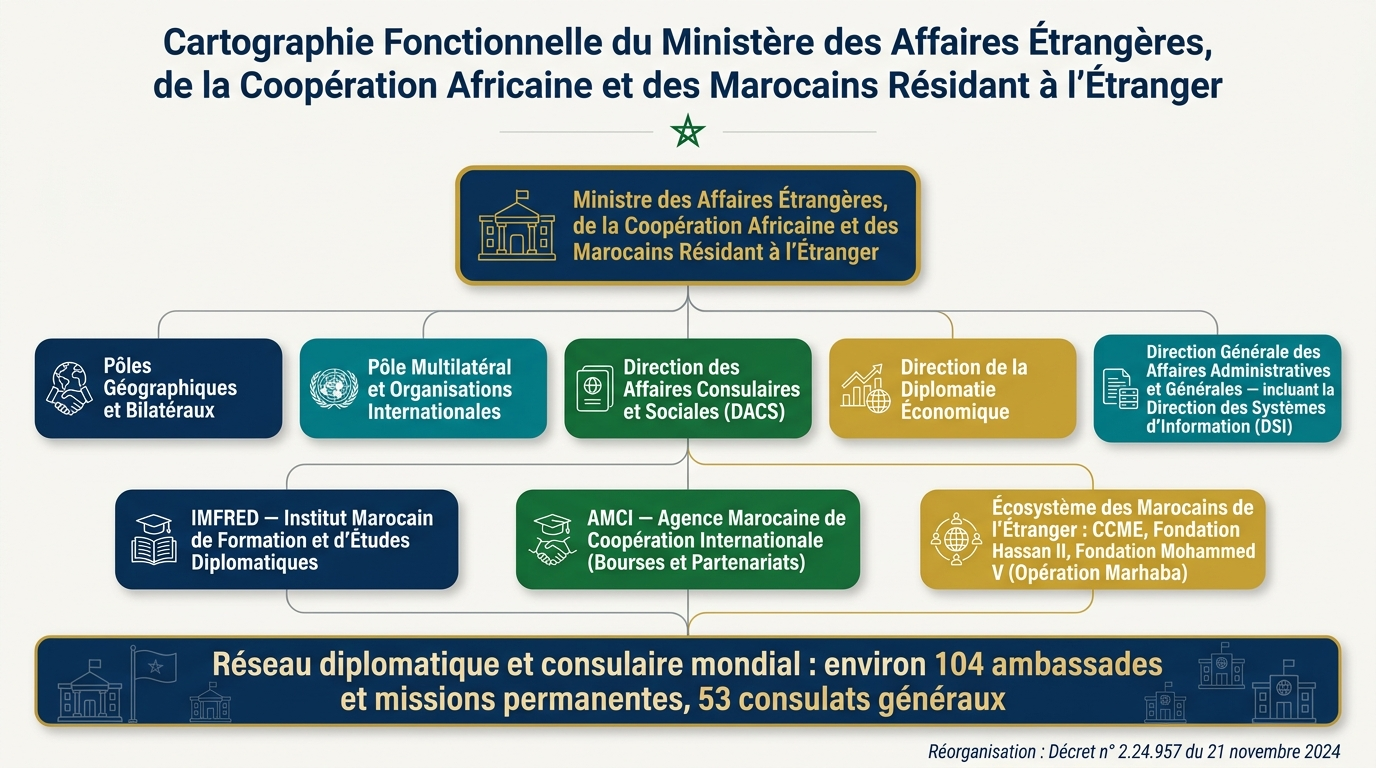
\includegraphics[width=\textwidth]{images/img_010_maecame_poles_organigramme.png}
    \caption{Cartographie fonctionnelle du MAECAME et de son écosystème}
\end{figure}}{}

% =========================================================================
\section{Fiche 2 : Les Constantes de la Politique Étrangère du Royaume}
% =========================================================================

\begin{enumerate}
    \item \textbf{Le Roi, chef de la diplomatie :} la Constitution de 2011 confie au Roi la représentation de l'État et la signature des traités (article 55) ; le préambule affirme l'appartenance du Maroc à l'Afrique, au monde arabo-islamique et à la Méditerranée, et son ouverture sur l'Europe et le monde.
    \item \textbf{La cause nationale :} l'intégrité territoriale et le dossier du Sahara marocain constituent « le prisme » à travers lequel le Royaume évalue ses partenariats (Discours de la Marche Verte 2022).
    \item \textbf{L'ancrage africain :} retour à l'Union Africaine (30 janvier 2017), diplomatie de coopération Sud-Sud, co-développement, Initiative Atlantique, gazoduc Nigeria-Maroc, Fondation Mohammed VI des Oulémas Africains, leadership royal sur la question migratoire.
    \item \textbf{La diversification des partenariats :} Europe (partenaire historique), États-Unis (allié majeur non-OTAN), Chine (partenariat stratégique 2016, Nouvelles Routes de la Soie), monde arabe et pays du Golfe, Amérique latine et Asie.
    \item \textbf{La diplomatie économique :} promotion des investissements, des exportations et de l'image du Royaume (Mondial 2030, énergies renouvelables, hydrogène vert, automobile, Tanger Med, port Dakhla Atlantique).
    \item \textbf{Le multilatéralisme et la crédibilité :} respect du droit international, contribution aux opérations de paix, présidence du Conseil des droits de l'homme en 2024, Pacte de Marrakech sur les migrations (2018), candidature au Conseil de sécurité pour 2028-2029.
    \item \textbf{La diplomatie de proximité :} protection et accompagnement des Marocains du monde, considérés comme partie intégrante de la Nation (articles 16 à 18 de la Constitution).
\end{enumerate}

\IfFileExists{images/img_004_constantes_politique_etrangere.png}{%
\begin{figure}[H]
    \centering
    
\includegraphics[width=\textwidth]{images/img_004_constantes_politique_etrangere.png}
    \caption{Les sept constantes de la politique étrangère du Royaume}
\end{figure}}{}

% =========================================================================
\section{Fiche 3 : Le Dossier du Sahara Marocain --- Chronologie et Position Internationale}
% =========================================================================

\begin{table}[H]
\centering
\small
\begin{tabular}{|p{3cm}|p{12.5cm}|}
\hline
\rowcolor{gray!20} \textbf{Date} & \textbf{Événement} \\ \hline
6 nov. 1975 & Marche Verte : 350 000 volontaires ; accords de Madrid (14 nov. 1975). \\ \hline
1991 & Cessez-le-feu et création de la MINURSO (Mission des Nations Unies pour l'organisation d'un référendum au Sahara occidental). \\ \hline
11 avril 2007 & Le Maroc présente l'\textbf{Initiative marocaine pour la négociation d'un statut d'autonomie} de la région du Sahara, qualifiée depuis de « sérieuse et crédible » par le Conseil de sécurité. \\ \hline
2015-2016 & Nouveau modèle de développement des provinces du Sud (77 milliards de dirhams), Discours de Laâyoune (6 nov. 2015). \\ \hline
10 déc. 2020 & Proclamation américaine reconnaissant la souveraineté du Maroc sur le Sahara ; réaffirmée par le secrétaire d'État Marco Rubio le 8 avril 2025. \\ \hline
18 mars 2022 & L'Espagne qualifie le plan d'autonomie de « base la plus sérieuse, réaliste et crédible » (lettre du président Sánchez). \\ \hline
30 juillet 2024 & Lettre du président Macron : « le présent et l'avenir du Sahara occidental s'inscrivent dans le cadre de la souveraineté marocaine » ; position réitérée devant le Parlement marocain le 29 octobre 2024. \\ \hline
1\textsuperscript{er} juin 2025 & Le Royaume-Uni juge le plan d'autonomie « la base la plus crédible, viable et pragmatique » (déclaration Lammy-Bourita). \\ \hline
31 oct. 2025 & \textbf{Résolution 2797} du Conseil de sécurité (11 voix pour, 3 abstentions : Chine, Russie, Pakistan ; l'Algérie ne participe pas au vote) : l'autonomie sous souveraineté marocaine est \textbf{la base} des négociations, « solution la plus réalisable » ; mandat de la MINURSO prorogé jusqu'au 31 octobre 2026. \\ \hline
29 janv. 2026 & 15\textsuperscript{e} Conseil d'association Maroc-UE : première position commune des 27 en faveur du plan d'autonomie, confirmée à Rabat le 16 avril 2026 par la Haute Représentante Kaja Kallas. \\ \hline
Fév. 2026 & Réunions de Madrid (8 février) puis de \textbf{Washington (23-24 février)} entre le Maroc, l'Algérie, la Mauritanie et le Polisario, sous l'égide des États-Unis et de l'Envoyé personnel Staffan de Mistura : premiers échanges directs depuis environ sept ans. \\ \hline
22 sept. 2026 & À l'Assemblée générale de l'ONU, M. Bourita énonce \textbf{six principes} (aucune solution hors de l'autonomie sous souveraineté marocaine ; négociation onusienne sur la seule base de l'initiative ; obligations de la résolution 2797 non négociables ; refus du statu quo ; crédibilité liée au respect du cessez-le-feu ; libération des populations de Tindouf). Prochaine échéance : nouvelle résolution avant le 31 octobre 2026. \\ \hline
\end{tabular}
\caption{Chronologie utile du dossier du Sahara marocain}
\end{table}

\IfFileExists{images/img_005_sahara_chronologie_soutiens.png}{%
\begin{figure}[H]
    \centering
    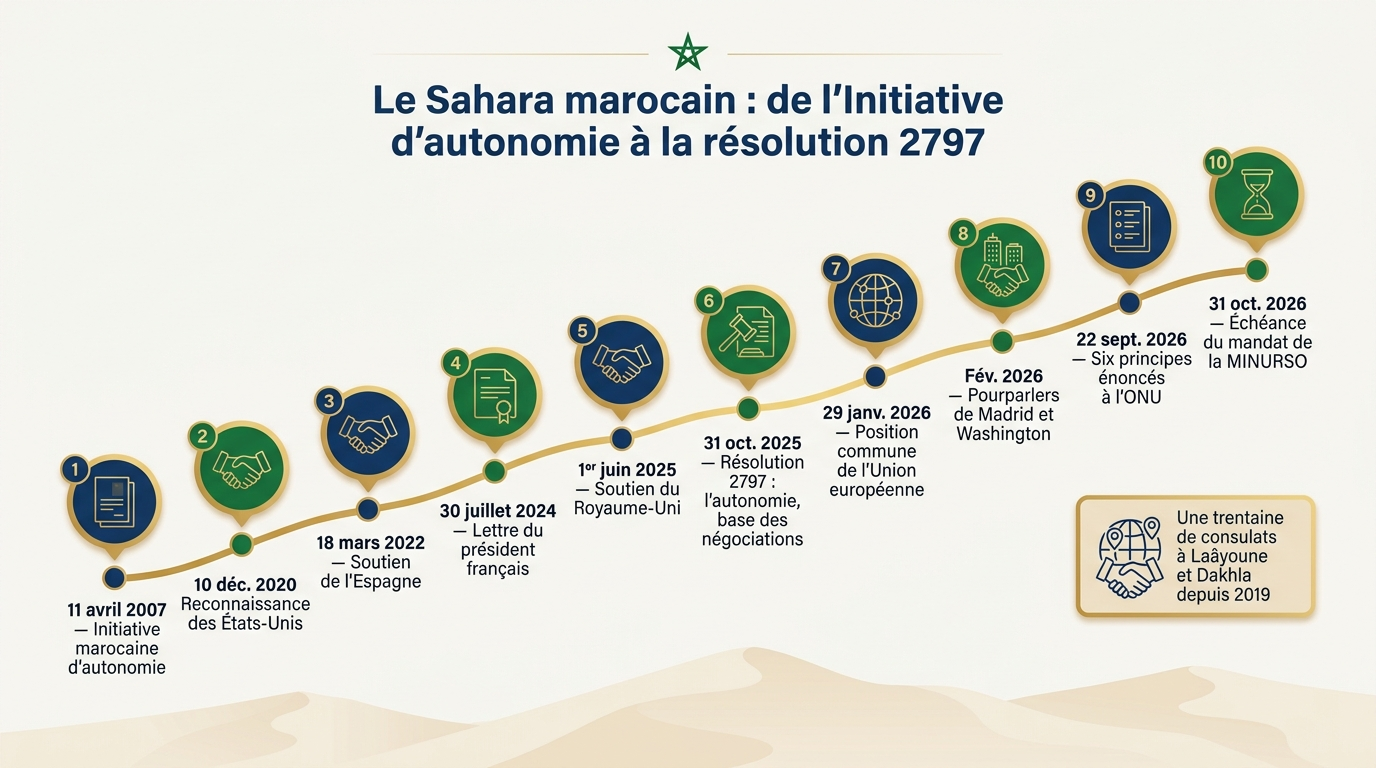
\includegraphics[width=\textwidth]{images/img_005_sahara_chronologie_soutiens.png}
    \caption{Frise du dossier du Sahara : de l'Initiative d'autonomie (2007) à la résolution 2797 (2025)}
\end{figure}}{}

% =========================================================================
\section{Fiche 4 : L'Ancrage Africain et les Grands Projets Structurants}
% =========================================================================

\begin{itemize}
    \item \textbf{Union Africaine :} retour du Maroc le 30 janvier 2017 (après 33 ans d'absence de l'OUA/UA depuis 1984). Demande d'adhésion à la \textbf{CEDEAO} le 24 février 2017, accord de principe le 4 juin 2017, toujours en attente.
    \item \textbf{Migration :} Sa Majesté le Roi désigné « Leader de l'Union Africaine sur la question de la migration » (janvier 2018) ; Pacte mondial de Marrakech (10-11 décembre 2018) ; \textbf{Observatoire Africain des Migrations} inauguré à Rabat le 18 décembre 2020.
    \item \textbf{Initiative Atlantique (novembre 2023) :} offrir aux pays du Sahel (Mali, Burkina Faso, Niger, Tchad) un accès à l'océan Atlantique via les infrastructures marocaines, notamment le \textbf{port Dakhla Atlantique} (environ 1,2 milliard d'euros, livraison attendue en 2028-2029).
    \item \textbf{Gazoduc Nigeria-Maroc (Gazoduc Africain Atlantique) :} environ 6 900 km, 25 milliards de dollars, 13 pays traversés ; accord intergouvernemental signé par les États de la CEDEAO au sommet de Freetown le 19 juillet 2026 ; décision finale d'investissement attendue, premier gaz vers 2031.
    \item \textbf{Coopération Sud-Sud :} AMCI (bourses, formation, expertise), OCP Africa et engrais, Banques marocaines présentes dans une trentaine de pays africains, Royal Air Maroc, Fondation Mohammed VI des Oulémas Africains (dahir du 24 juin 2015, 48 sections nationales fin 2024), Institut Mohammed VI de formation des imams.
    \item \textbf{ZLECAf :} Zone de libre-échange continentale africaine (accord de Kigali, 2018 ; entrée en vigueur 2019) ; le Maroc l'a ratifiée et y voit un levier d'intégration industrielle.
    \item \textbf{Coupe du monde 2030 :} attribuée le 11 décembre 2024 au trio Maroc-Espagne-Portugal (13 juin -- 21 juillet 2030), vitrine de la diplomatie sportive et économique.
\end{itemize}

\IfFileExists{images/img_006_afrique_initiative_atlantique_gazoduc.png}{%
\begin{figure}[H]
    \centering
    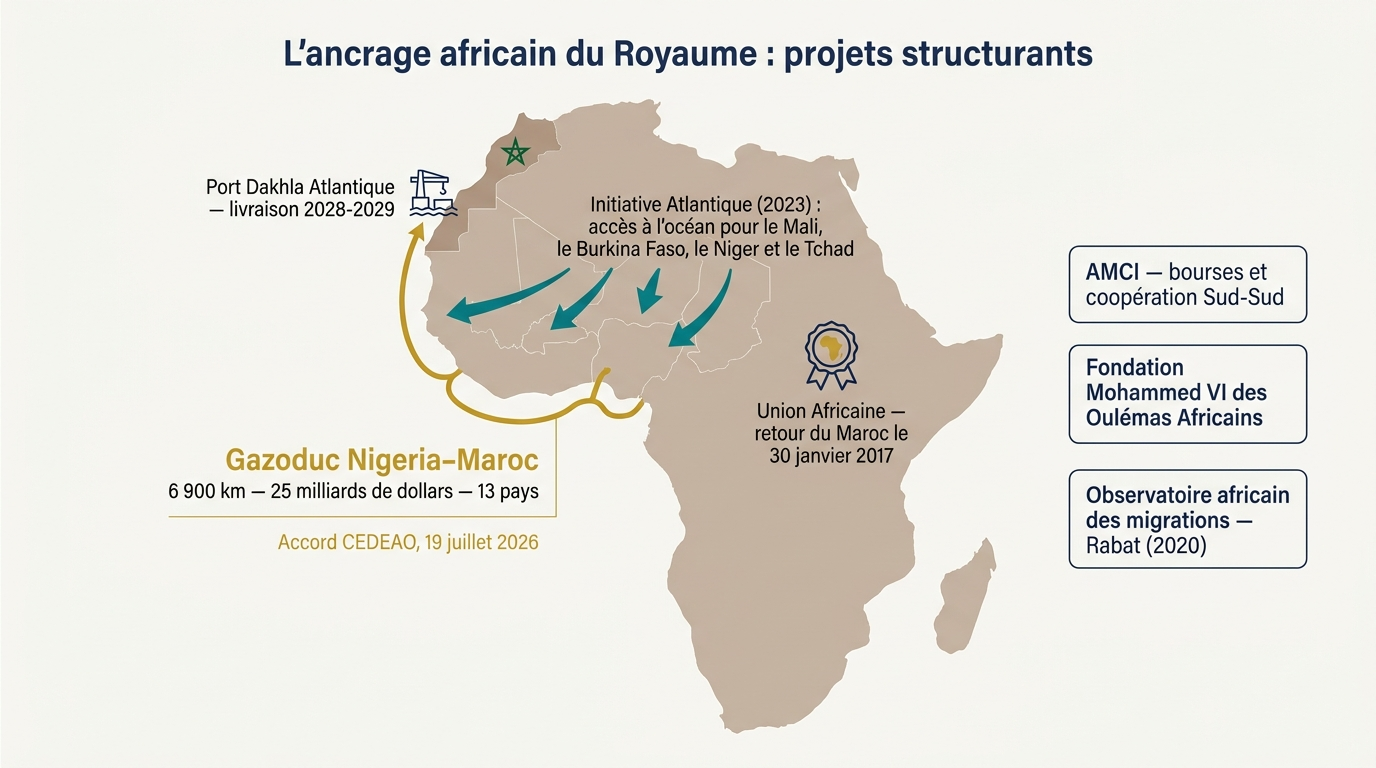
\includegraphics[width=\textwidth]{images/img_006_afrique_initiative_atlantique_gazoduc.png}
    \caption{Carte des projets structurants de l'ancrage africain : Initiative Atlantique et gazoduc Nigeria--Maroc}
\end{figure}}{}

% =========================================================================
\section{Fiche 5 : Les Marocains du Monde --- Chiffres et Politique Publique}
% =========================================================================

\begin{table}[H]
\centering
\small
\begin{tabular}{|p{5cm}|p{4cm}|p{6.5cm}|}
\hline
\rowcolor{gray!20} \textbf{Indicateur} & \textbf{Valeur} & \textbf{Observation} \\ \hline
Effectif des MRE & « Plus de 5 millions » & Chiffre officiel prudent ; la presse évoque souvent 6 millions. Seule statistique exacte : les immatriculés consulaires. \\ \hline
Transferts 2024 & 117,7 MMDH (+2,1 \%) & Soit 7,7 \% du PIB ; ils étaient de 57,4 MMDH en 2014 (doublement en dix ans). \\ \hline
Transferts 2025 & Plus de 122 MMDH (+2,6 \%) & Première source de devises avec le tourisme et les phosphates ; stabilisent les réserves de change. \\ \hline
Transferts à fin juillet 2026 & 74,78 MMDH (+8,1 \%) & Dynamique soutenue en 2026. \\ \hline
Opération Marhaba 2026 & 4 137 594 MRE accueillis (+1,8 \%) & Du 10 juin au 15 septembre ; 26 espaces d'accueil, 1 134 assistantes sociales, pics d'environ 80 000 arrivées par jour (Fondation Mohammed V pour la Solidarité). \\ \hline
Participation politique 2026 & Vote par procuration dématérialisé & Plateforme « E-procuration » (24 août -- 22 septembre 2026) ; pas de bureaux de vote à l'étranger ni de sièges réservés. \\ \hline
\end{tabular}
\caption{Tableau de bord des Marocains du monde}
\end{table}

\begin{tcolorbox}[colback=yellow!5!white,colframe=orange!75!black,title=\textbf{La réforme des institutions des MRE (Discours de la Marche Verte, 6 novembre 2024)}]
\begin{itemize}
    \item \textbf{Constat royal :} dispersion des intervenants, résultats insuffisants malgré les moyens ; nécessité d'une « refonte globale ».
    \item \textbf{Deux piliers :} (1) le \textbf{CCME} recentré sur la réflexion stratégique et la prospective ; (2) une nouvelle \textbf{Fondation Mohammedia des MRE}, bras opérationnel qui regroupe les attributions dispersées (dont celles de la Fondation Hassan II).
    \item \textbf{Mécanisme national de mobilisation des compétences} des Marocains du monde (médecins, ingénieurs, chercheurs, entrepreneurs) au service du développement.
    \item \textbf{État d'avancement :} en septembre 2026, les textes créant la Fondation n'ont pas encore été adoptés : parler d'une réforme « en cours de mise en œuvre ».
    \item \textbf{Cadre constitutionnel :} articles 16 (protection des droits et intérêts des MRE), 17 (droits de citoyenneté, dont le vote) et 18 (participation aux institutions consultatives) de la Constitution de 2011.
\end{itemize}
\end{tcolorbox}

\IfFileExists{images/img_007_mre_transferts_marhaba_reforme.png}{%
\begin{figure}[H]
    \centering
    
\includegraphics[width=\textwidth]{images/img_007_mre_transferts_marhaba_reforme.png}
    \caption{Marocains du monde : transferts, opération Marhaba et refonte institutionnelle}
\end{figure}}{}

% =========================================================================
\section{Fiche 6 : Partenariats Stratégiques et Actualité 2024-2026}
% =========================================================================

\begin{itemize}
    \item \textbf{Union européenne :} premier partenaire commercial ; statut avancé (2008). Arrêt de la Cour de justice de l'UE du 4 octobre 2024 annulant les accords agricole et de pêche ; nouvel accord agricole par échange de lettres publié au Journal officiel de l'UE le 3 octobre 2025 (application provisoire) ; pas de nouvel accord de pêche à ce jour. Position commune des 27 sur l'autonomie (janvier 2026).
    \item \textbf{États-Unis :} accord de libre-échange (2006), allié majeur non-OTAN, exercice African Lion, reconnaissance de la souveraineté sur le Sahara (2020, réaffirmée en 2025), médiation des pourparlers de Washington (février 2026).
    \item \textbf{Espagne et France :} partenaires historiques ; co-organisation du Mondial 2030 avec l'Espagne ; visite d'État du président Macron (octobre 2024) et « partenariat d'exception renforcé ».
    \item \textbf{Israël :} déclaration tripartite du 22 décembre 2020 ; le 16 septembre 2026 à New York, accord pour élever les bureaux de liaison au rang d'\textbf{ambassades} et échanger des ambassadeurs, avec accords d'investissement et de double imposition avant fin 2026. Le Maroc défend l'État palestinien dans les frontières de 1967 avec Al-Qods-Est pour capitale et préside le Comité Al-Qods.
    \item \textbf{Gaza :} accord de participation du Maroc à la Force internationale de stabilisation signé à Rabat le 15 juillet 2026 ; Maroc membre fondateur du Conseil de paix.
    \item \textbf{Chine :} partenariat stratégique (mai 2016), premier pays maghrébin signataire des Nouvelles Routes de la Soie (novembre 2017), plan de mise en œuvre conjoint (5 janvier 2022) ; investissements dans l'automobile électrique et les batteries.
    \item \textbf{Algérie :} rupture des relations diplomatiques le 24 août 2021, fermeture de l'espace aérien (septembre 2021), non-renouvellement du gazoduc Maghreb-Europe (octobre 2021), frontières terrestres fermées depuis 1994 ; présence algérienne aux pourparlers de 2026. Position marocaine constante : la main tendue (discours royaux de 2018, 2021 et 2022).
    \item \textbf{Multilatéral :} membre du Conseil des droits de l'homme 2023-2025, \textbf{présidence en 2024} (ambassadeur Omar Zniber) ; candidature au \textbf{Conseil de sécurité 2028-2029} (dernier mandat 2012-2013), soutenue par le Sommet arabe de Bagdad (mai 2025).
\end{itemize}

% =========================================================================
\section{Fiche 7 : Le Numérique au Service de la Diplomatie et des Services Consulaires}
% =========================================================================

\begin{itemize}
    \item \textbf{e-Visa :} lancé le 10 juillet 2022 (plateforme acces-maroc.ma) ; visa électronique en 72 heures (24 heures en express), valable 30 jours ; \textbf{385 738 e-visas} délivrés à fin 2024, à 95 \% pour le tourisme, 111 nationalités (l'Inde en tête).
    \item \textbf{Services consulaires en ligne :} portail \texttt{consulat.ma} (guide des services), \texttt{rdv.consulat.ma} (prise de rendez-vous), plateforme interne \textbf{eConsulat} enrichie de nouveaux modules (rapatriement des dépouilles, authentification des permis de conduire, échanges avec le ministère de la Justice) ; objectif de temps d'attente ramené de 45 minutes (2025) à 38 minutes (2026).
    \item \textbf{Apostille :} adhésion du Maroc à la Convention de La Haye (en vigueur le 14 août 2016), demande en ligne sur \texttt{apostille.ma} : simplification de la légalisation des documents pour les MRE et les investisseurs.
    \item \textbf{Cadre de sécurité :} loi 05-20 sur la cybersécurité et son décret 2-21-406 (15 juillet 2021) ; DGSSI (Administration de la Défense Nationale) ; \textbf{Stratégie nationale de cybersécurité 2030} (juillet 2024 : 4 piliers, 11 objectifs, 26 initiatives, 60 actions) ; loi 09-08 et CNDP pour les données personnelles, particulièrement sensibles pour un réseau de 150 postes à l'étranger.
    \item \textbf{Enjeux pour l'ingénieur d'État :} interopérabilité entre consulats, état civil et administrations nationales (RNP, Justice, Intérieur), continuité de service sur des fuseaux horaires multiples, protection des données des Marocains du monde, lutte contre la fraude documentaire (biométrie), communication numérique et image du Royaume, données au service de la diplomatie économique.
\end{itemize}

\IfFileExists{images/img_008_services_consulaires_numeriques.png}{%
\begin{figure}[H]
    \centering
    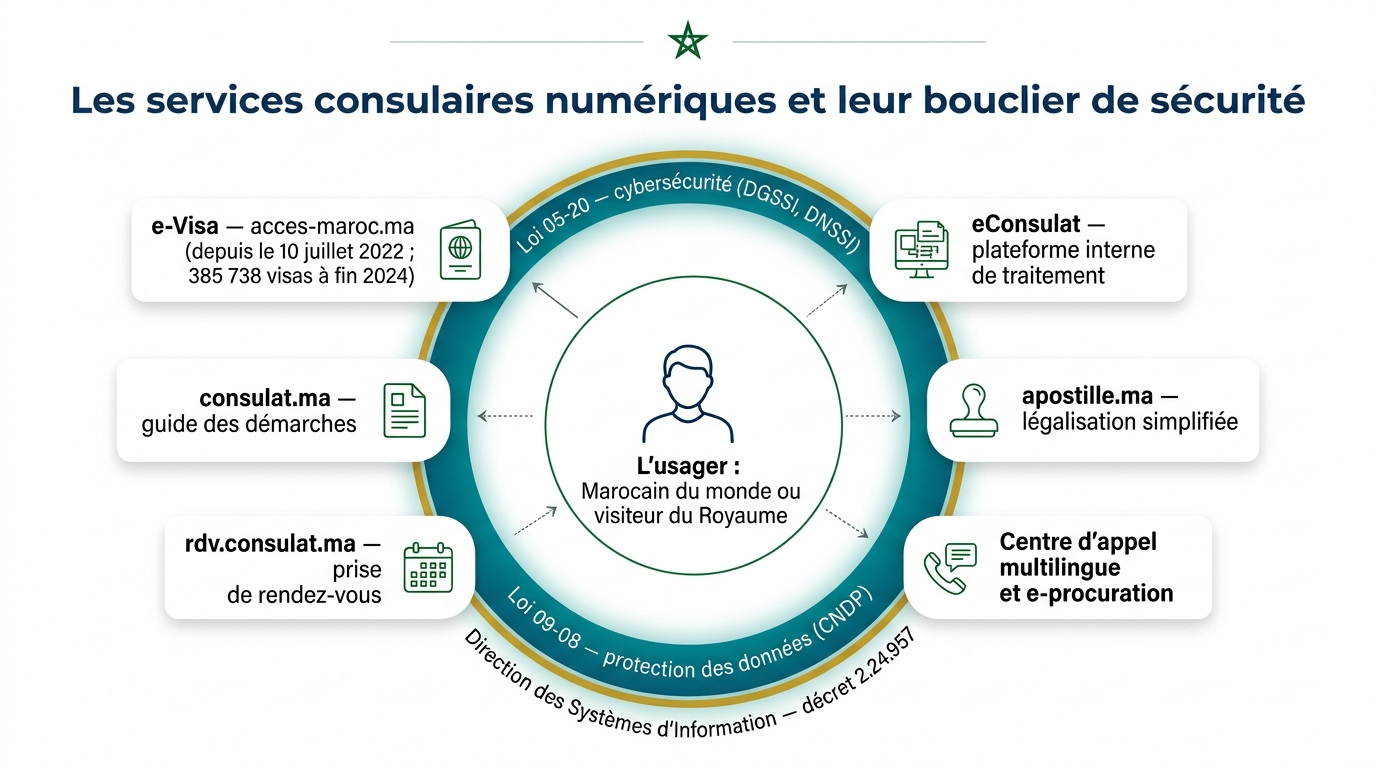
\includegraphics[width=\textwidth]{images/img_008_services_consulaires_numeriques.png}
    \caption{Écosystème numérique des services consulaires : e-Visa, eConsulat, apostille et sécurité des données}
\end{figure}}{}

% =========================================================================
\section{Fiche 8 : Chiffres et Dates à Retenir par Cœur}
% =========================================================================

\begin{multicols}{2}
\small
\begin{itemize}
    \item \textbf{1956 :} création du ministère.
    \item \textbf{1975 :} Marche Verte (6 novembre).
    \item \textbf{1984 :} retrait de l'OUA ; \textbf{2017 :} retour à l'UA (30 janvier).
    \item \textbf{2007 :} Initiative d'autonomie (11 avril) ; création du CCME.
    \item \textbf{2011 :} Constitution (articles 16-18 sur les MRE, article 55 sur les traités).
    \item \textbf{2016 :} partenariat stratégique avec la Chine ; apostille en vigueur.
    \item \textbf{2018 :} Pacte de Marrakech sur les migrations ; Roi leader UA migration.
    \item \textbf{2020 :} reconnaissance américaine (10 décembre) ; Observatoire africain des migrations (18 décembre).
    \item \textbf{2022 :} lancement de l'e-Visa (10 juillet) ; Espagne soutient l'autonomie.
    \item \textbf{2023 :} Initiative Atlantique (novembre).
    \item \textbf{2024 :} lettre Macron (30 juillet) ; présidence du CDH ; décret 2.24.957 de réorganisation ; Discours MRE (6 novembre) ; Mondial 2030 attribué (11 décembre).
    \item \textbf{2025 :} Royaume-Uni (1\textsuperscript{er} juin) ; résolution 2797 (31 octobre) ; transferts MRE $>$ 122 MMDH.
    \item \textbf{2026 :} position UE (29 janvier) ; pourparlers de Washington (février) ; accord gazoduc CEDEAO (19 juillet) ; ambassades Maroc-Israël (16 septembre) ; six principes à l'ONU (22 septembre) ; échéance MINURSO (31 octobre).
    \item \textbf{Réseau :} environ 104 ambassades, 53 consulats généraux.
    \item \textbf{MRE :} plus de 5 millions ; 117,7 MMDH en 2024 (7,7 \% du PIB) ; 4,14 millions accueillis par Marhaba 2026.
    \item \textbf{Gazoduc :} 6 900 km, 25 milliards de dollars, 13 pays.
    \item \textbf{e-Visa :} 385 738 délivrés à fin 2024.
\end{itemize}
\end{multicols}


% --- TROISIÈME PARTIE : STRATÉGIE JOUR J ET PLANNING D'URGENCE ---
\part{STRATÉGIE JOUR J ET PLANNING D'URGENCE}

\chapter{Planning d'Urgence Commando : J-4 jusqu'au 27 Septembre}

Avec quatre jours avant les épreuves écrites du \textbf{dimanche 27 septembre 2026} (présence à \textbf{7h30} à la \textbf{FSJES de Salé}, route Outa Hssain, Salé El Jadida, avec la CIN), la stratégie est celle du \textbf{haut rendement ciblé}. Le barème impose les priorités : l'épreuve de \textbf{spécialité informatique et réseaux (3 h, coefficient 4)} pèse deux fois plus que la \textbf{rédaction sur les attributions du ministère (2 h, coefficient 2)}. Il faut donc consacrer environ 60 \% du temps à la spécialité (réseaux et télécommunications en priorité, développement ensuite) et 40 \% à la matière diplomatique, tout en capitalisant sur la méthode acquise pour le MEF (plan binaire, introduction en 5 étapes).

\begin{tcolorbox}[colback=blue!5!white,colframe=blue!75!black,title=\textbf{Ce qui est déjà acquis (ne pas y repasser du temps)}]
La méthodologie de la dissertation (à recaler sur 2 heures), la structure en deux parties, le socle informatique général (algorithmique, SQL, POO, cybersécurité, data) et la culture économique générale (PIB, déficit, dette, inflation). Une relecture rapide suffit ; l'effort nouveau porte sur les réseaux et télécommunications, qui n'étaient qu'un bloc parmi d'autres au MEF et deviennent ici la spécialité la plus dotée (10 postes sur 16).
\end{tcolorbox}

\section{Le Programme Heure par Heure (Sprint Final)}

\begin{table}[H]
\centering
\small
\begin{tabular}{|p{3cm}|p{3.5cm}|p{8.5cm}|}
\hline
\rowcolor{gray!20} \textbf{Jour / Date} & \textbf{Créneau Horaire} & \textbf{Objectif Haute Rentabilité} \\ \hline
\multirow{2}{*}{\textbf{J-4 : 23 Sept.}} & 15h00 - 19h00 & \textbf{Bloc 1 : Cadrage du concours et fondamentaux de la diplomatie marocaine} \newline Lire l'introduction et le chapitre 1 (les trois épreuves, barème, attentes du jury). Mémoriser la Fiche 1 (organisation du MAECAME) et la Fiche 2 (constantes de la politique étrangère). \\ \cline{2-3}
& 20h00 - 23h00 & \textbf{Bloc 2 : Spécialité --- Réseaux et télécommunications (1)} \newline Modèle OSI/TCP-IP, adressage et sous-réseaux (exercices de calcul), routage, VLAN, VPN, Wi-Fi, sécurité périmétrique. Traiter les exercices rédigés du chapitre 3 (architecture réseau d'une ambassade). \\ \hline

\multirow{3}{*}{\textbf{J-3 : 24 Sept.}} & 08h30 - 12h30 & \textbf{Bloc 3 : Spécialité --- Développement et bases de données} \newline POO, architecture web et API, SQL et Merise (exercice de conception d'un système de rendez-vous consulaire), génie logiciel, sécurité applicative (OWASP). \\ \cline{2-3}
& 14h00 - 18h00 & \textbf{Bloc 4 : Sahara, Afrique et Marocains du monde} \newline Fiches 3, 4 et 5 : chronologie du Sahara et résolution 2797, retour à l'UA, Initiative Atlantique, gazoduc, chiffres MRE et réforme de 2024. Lire les Sujets 1 à 3 du chapitre 2. \\ \cline{2-3}
& 19h00 - 22h30 & \textbf{Bloc 5 : Simulation de la rédaction en 2 h chrono} \newline Rédiger un sujet du chapitre 2 \textbf{sans regarder la copie modèle}, puis se corriger avec la grille. Ensuite, lire les Sujets 4 à 6 (diplomatie économique, numérique consulaire, multilatéralisme). \\ \hline

\multirow{3}{*}{\textbf{J-2 : 25 Sept.}} & 09h00 - 12h30 & \textbf{Bloc 6 : Spécialité --- Réseaux et télécommunications (2)} \newline Télécoms (fibre, 4G/5G, VoIP, liaisons satellitaires pour les postes isolés), supervision, haute disponibilité, PRA/PCA, cybersécurité (loi 05-20, DNSSI, ISO 27001). Refaire les calculs de sous-réseaux. \\ \cline{2-3}
& 14h30 - 17h30 & \textbf{Bloc 7 : Banque de questions ministère et diplomatie} \newline Parcourir toutes les questions 🔴 et 🟠 du chapitre 3 en cachant les réponses ; relire les Fiches 6 et 7. \\ \cline{2-3}
& 18h30 - 21h00 & \textbf{Bloc 8 : Examen blanc complet (chapitre 6)} \newline Épreuve de spécialité (3 h) puis, après une pause, la rédaction (2 h) ; autocorrection avec les grilles. \\ \hline

\multirow{2}{*}{\textbf{J-1 : 26 Sept.}} & 09h00 - 12h00 & \textbf{Bloc 9 : Fiches chiffres clés et phrases d'accroche} \newline Mémoriser la Fiche 8 (dates et chiffres), les pièges du chapitre 3 et préparer 5 accroches réutilisables (discours royaux, résolution 2797, Constitution). \\ \cline{2-3}
& 14h00 - 17h00 & \textbf{Bloc 10 : Préparation matérielle et sérénité} \newline CIN obligatoire (l'annonce officielle tient lieu de convocation), numéro de salle et de siège notés, stylos, montre analogique, calculatrice simple si autorisée, trajet vers la FSJES de Salé repéré. \textbf{Arrêt complet des révisions à 18h00.} \\ \hline

\textbf{Jour J : 27 Sept.} & 07h30 & \textbf{Épreuves écrites à la FSJES de Salé} \newline Arrivée à 7h00. Spécialité (3 h) : lire tout le sujet, traiter d'abord les questions sûres, garder 15 minutes de relecture. Rédaction (2 h) : timing 10m / 20m / 10m / 70m / 10m. \\ \hline
\end{tabular}
\caption{Planning intensif d'urgence J-4}
\end{table}

\IfFileExists{images/img_012_planning_commando_j4_matrice.png}{%
\begin{figure}[H]
    \centering
    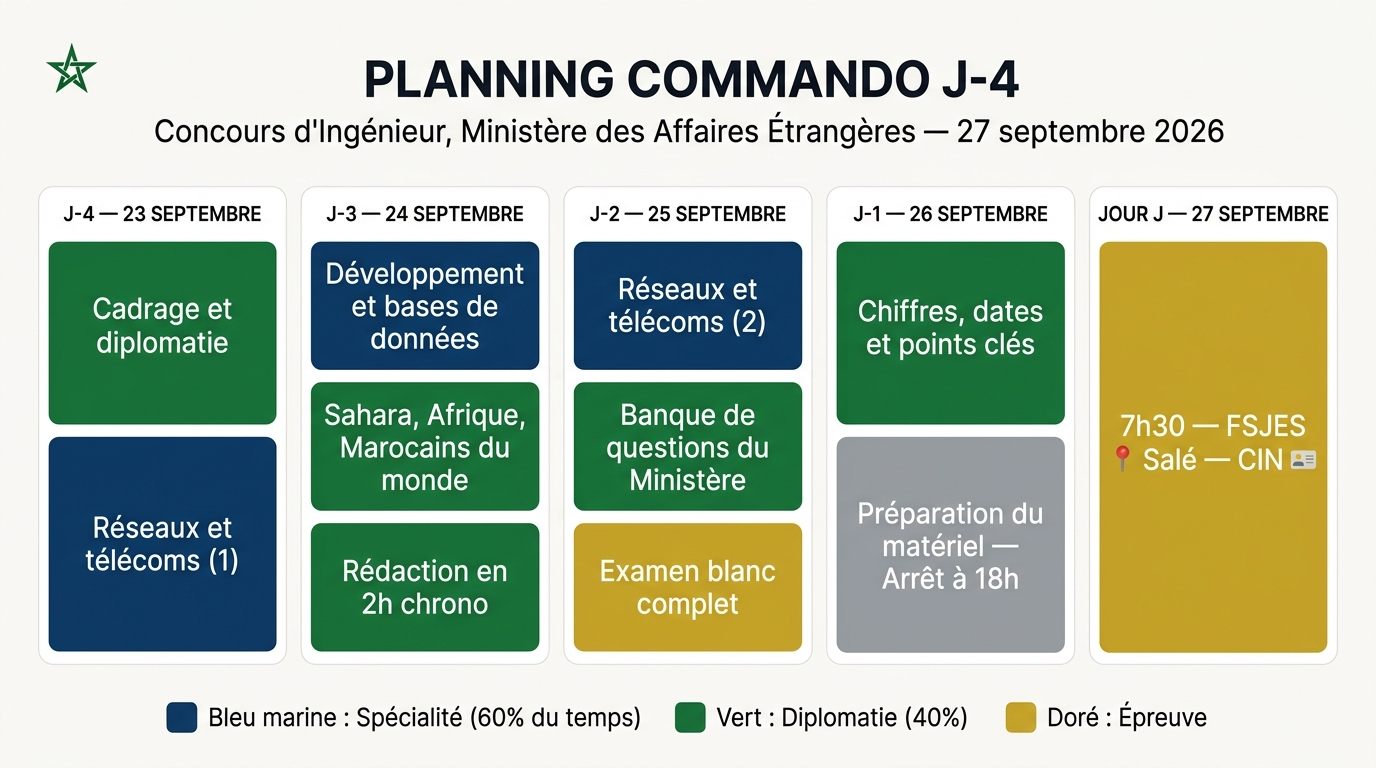
\includegraphics[width=\textwidth]{images/img_012_planning_commando_j4_matrice.png}
    \caption{Matrice d'urgence des 4 jours avant l'épreuve du 27 septembre}
\end{figure}}{}

\section{Checklist Finale pour le Jour J}
\begin{enumerate}
    \item \textbf{Vocabulaire valorisé :} \textit{intégrité territoriale, plan d'autonomie, diplomatie économique, coopération Sud-Sud, partenariat gagnant-gagnant, co-développement, voisinage, multilatéralisme, diplomatie de proximité au service des Marocains du monde, souveraineté numérique, protection des données.}
    \item \textbf{Références à mobiliser :} discours royaux (Marche Verte, Trône, Révolution du Roi et du Peuple), Constitution de 2011 (préambule sur l'appartenance africaine et arabo-islamique, articles 16 à 18 sur les MRE), résolutions du Conseil de sécurité, Acte constitutif de l'Union Africaine.
    \item \textbf{Posture d'ingénieur d'État :} montrer que la technologie sert la diplomatie : services consulaires numériques, sécurité des systèmes d'information, données des Marocains du monde, communication et image du Royaume.
    \item \textbf{Neutralité et rigueur :} ton institutionnel, pas de polémique, pas de chiffre inventé ; en cas de doute, formuler avec prudence (« selon les données officielles récentes »).
\end{enumerate}

\chapter{Examen Blanc Chronométré (Conditions Réelles)}

\begin{tcolorbox}[colback=red!4!white,colframe=red!60!black,title=\textbf{Consignes de l'examen blanc}]
\begin{itemize}
    \item Reproduire la journée du 27 septembre : \textbf{Épreuve A --- Spécialité (3 heures)}, pause, puis \textbf{Épreuve B --- Rédaction (2 heures)}.
    \item Répondre sur feuille, \textbf{sans consulter les corrigés}, placés sur des pages séparées.
    \item Épreuve A : partie 1 = 30 QCM (une seule bonne réponse, 0,5 point chacun, 15 points) ; partie 2 = 3 exercices rédigés (25 points). Total sur 40, ramené sur 20.
    \item Épreuve B : sujet unique, noté sur 20 avec la grille du chapitre 1.
    \item Objectif de sécurité : au moins 12/20 à chaque épreuve.
\end{itemize}
\end{tcolorbox}

% =========================================================================
\section{Épreuve A --- Spécialité Informatique et Réseaux (3 heures, coefficient 4)}
% =========================================================================

\subsection*{Partie 1 : 30 QCM (45 minutes)}

\begin{enumerate}[leftmargin=*, label=\textbf{Q\arabic*.}]
    \item Un réseau /27 offre combien d'adresses hôtes utilisables ?
    \newline (A) 14 \quad (B) 30 \quad (C) 32 \quad (D) 62
    \item À quelle couche du modèle OSI fonctionne un commutateur (switch) classique ?
    \newline (A) 1 \quad (B) 2 \quad (C) 3 \quad (D) 4
    \item Quel protocole évite les boucles de commutation ?
    \newline (A) OSPF \quad (B) STP \quad (C) DHCP \quad (D) SNMP
    \item Quel protocole de routage est utilisé entre systèmes autonomes sur Internet ?
    \newline (A) RIP \quad (B) OSPF \quad (C) BGP \quad (D) EIGRP
    \item Dans IPsec, quel protocole assure le chiffrement des données ?
    \newline (A) AH \quad (B) ESP \quad (C) IKE \quad (D) GRE
    \item Quelle norme permet le transport de plusieurs VLAN sur un même lien ?
    \newline (A) 802.11ax \quad (B) 802.1X \quad (C) 802.1Q \quad (D) 802.3
    \item Quel mécanisme authentifie individuellement un poste avant l'accès au réseau filaire ou Wi-Fi ?
    \newline (A) NAT \quad (B) 802.1X avec RADIUS \quad (C) WEP \quad (D) DNS
    \item Quel est le port par défaut de SSH ?
    \newline (A) 21 \quad (B) 22 \quad (C) 23 \quad (D) 25
    \item Quelle adresse est une adresse IPv4 privée ?
    \newline (A) 8.8.8.8 \quad (B) 172.20.5.1 \quad (C) 41.140.0.1 \quad (D) 200.1.1.1
    \item Pour la voix sur IP, quel protocole établit et termine les appels ?
    \newline (A) RTP \quad (B) SIP \quad (C) SMTP \quad (D) FTP
    \item Quelle fibre optique convient aux liaisons de plusieurs dizaines de kilomètres ?
    \newline (A) Multimode \quad (B) Monomode \quad (C) Cuivre catégorie 6 \quad (D) Coaxial
    \item Un SLA de 99,9 \% tolère une indisponibilité annuelle d'environ :
    \newline (A) 5 minutes \quad (B) 53 minutes \quad (C) 8 h 45 \quad (D) 3 jours 15 h
    \item Quel protocole sert à superviser les équipements réseau ?
    \newline (A) SNMP \quad (B) SIP \quad (C) LDAP \quad (D) NTP
    \item Quelle technologie opérateur fournit des réseaux privés virtuels multi-sites avec qualité de service garantie ?
    \newline (A) ADSL \quad (B) MPLS \quad (C) Wi-Fi 6 \quad (D) Bluetooth
    \item Que désigne le RTO dans un plan de reprise d'activité ?
    \newline (A) La perte de données maximale \quad (B) La durée maximale d'interruption \quad (C) Le coût du plan \quad (D) La fréquence des tests
    \item En SQL, quelle clause filtre les résultats d'une agrégation ?
    \newline (A) WHERE \quad (B) HAVING \quad (C) ORDER BY \quad (D) LIMIT
    \item Quelle forme normale exige que chaque attribut non-clé dépende de toute la clé primaire ?
    \newline (A) 1FN \quad (B) 2FN \quad (C) 3FN \quad (D) BCNF
    \item Une association « plusieurs à plusieurs » entre deux entités se traduit en relationnel par :
    \newline (A) une clé étrangère dans l'une des tables \quad (B) une table de jointure \quad (C) une vue \quad (D) un index
    \item Quel principe de la POO consiste à masquer les données derrière des méthodes ?
    \newline (A) Héritage \quad (B) Polymorphisme \quad (C) Encapsulation \quad (D) Surcharge
    \item Quel code HTTP signifie « ressource créée » ?
    \newline (A) 200 \quad (B) 201 \quad (C) 404 \quad (D) 500
    \item Dans une API REST, quelle méthode HTTP est utilisée pour supprimer une ressource ?
    \newline (A) GET \quad (B) POST \quad (C) PUT \quad (D) DELETE
    \item Quelle est la complexité moyenne du tri fusion ?
    \newline (A) $O(n)$ \quad (B) $O(n \log n)$ \quad (C) $O(n^2)$ \quad (D) $O(\log n)$
    \item Quelle structure de données fonctionne en FIFO ?
    \newline (A) Pile \quad (B) File \quad (C) Arbre binaire \quad (D) Table de hachage
    \item Que fait la commande Linux \texttt{chmod 750 script.sh} ?
    \newline (A) rwxr-x--- \quad (B) rw-r--r-- \quad (C) rwxrwxrwx \quad (D) r-x------
    \item Quel algorithme est asymétrique ?
    \newline (A) AES \quad (B) RSA \quad (C) SHA-256 \quad (D) 3DES
    \item Quelle attaque consiste à insérer du code SQL via un formulaire ?
    \newline (A) XSS \quad (B) CSRF \quad (C) Injection SQL \quad (D) DDoS
    \item Quel texte marocain régit la cybersécurité ?
    \newline (A) Loi 09-08 \quad (B) Loi 05-20 \quad (C) Loi 43-20 \quad (D) Loi 55-19
    \item Quelle norme définit un système de management de la sécurité de l'information ?
    \newline (A) ISO 9001 \quad (B) ISO/IEC 27001 \quad (C) ITIL \quad (D) COBIT
    \item Que signifie ETL ?
    \newline (A) Extract, Transform, Load \quad (B) Encrypt, Transfer, Log \quad (C) Edit, Test, Launch \quad (D) Export, Table, List
    \item Un conteneur Docker, par rapport à une machine virtuelle :
    \newline (A) embarque son propre noyau \quad (B) partage le noyau de l'hôte \quad (C) est toujours plus lent \quad (D) nécessite un hyperviseur de type 1
\end{enumerate}

\subsection*{Partie 2 : Exercices Rédigés (2 h 15)}

\begin{tcolorbox}[colback=blue!5!white,colframe=blue!75!black,title=\textbf{Exercice 1 --- Adressage et segmentation (9 points)}]
Le consulat général du Maroc dans une grande ville dispose du bloc \texttt{192.168.40.0/24}. Il doit accueillir : 50 postes de guichet et back-office, 20 téléphones IP, 6 serveurs locaux, 10 caméras et équipements techniques, un Wi-Fi visiteurs de 25 clients et une liaison point à point vers le routeur de secours 4G.
\begin{enumerate}
    \item Proposez un découpage VLSM (réseau, masque, plage, diffusion) en justifiant l'ordre d'allocation. (5 pts)
    \item Indiquez pour chaque sous-réseau le VLAN associé et les règles de filtrage principales. (2 pts)
    \item Le consulat souhaite passer en double pile IPv6 : donnez un exemple d'adressage IPv6 pour deux VLAN à partir du préfixe \texttt{2001:db8:40::/48} et expliquez l'intérêt. (2 pts)
\end{enumerate}
\end{tcolorbox}

\begin{tcolorbox}[colback=blue!5!white,colframe=blue!75!black,title=\textbf{Exercice 2 --- Base de données du suivi des demandes de visa (8 points)}]
On souhaite concevoir la base d'un système de traitement des demandes de visa électronique. Un demandeur (passeport unique, nationalité) dépose des demandes ; chaque demande concerne un type de visa (tourisme, affaires, études), est traitée par un agent d'un consulat ou du service central, et passe par des statuts datés (déposée, en instruction, acceptée, refusée, délivrée).
\begin{enumerate}
    \item Proposez le MCD (entités, associations, cardinalités). (3 pts)
    \item Déduisez le MLD. (2 pts)
    \item Écrivez la requête SQL donnant, pour chaque type de visa, le nombre de demandes acceptées et le délai moyen (en jours) entre le dépôt et l'acceptation pour l'année 2026. (3 pts)
\end{enumerate}
\end{tcolorbox}

\begin{tcolorbox}[colback=blue!5!white,colframe=blue!75!black,title=\textbf{Exercice 3 --- Sécurisation d'une plateforme exposée sur Internet (8 points)}]
La plateforme de rendez-vous consulaire subit des ralentissements et l'on soupçonne une exploitation automatisée des créneaux par des revendeurs, ainsi que des tentatives d'attaque.
\begin{enumerate}
    \item Décrivez l'architecture de sécurité que vous mettez en place devant et autour de l'application (au moins six composants ou mesures, justifiés). (4 pts)
    \item Proposez des mesures fonctionnelles et techniques contre la réservation automatisée et la revente de créneaux. (2 pts)
    \item Quelles obligations légales marocaines s'appliquent aux données traitées et à la gestion d'un incident ? (2 pts)
\end{enumerate}
\end{tcolorbox}

\newpage
% =========================================================================
\section{Corrigé de l'Épreuve A}
% =========================================================================

\subsection*{Corrigé des 30 QCM}
{\small
\begin{longtable}{|c|>{\raggedright\arraybackslash}p{4.6cm}|p{9.2cm}|}
\hline
\rowcolor{gray!20} \textbf{Q} & \textbf{Bonne réponse} & \textbf{Explication courte} \\ \hline
\endfirsthead
\hline
\rowcolor{gray!20} \textbf{Q} & \textbf{Bonne réponse} & \textbf{Explication courte} \\ \hline
\endhead
1 & B --- 30 & $2^{5} - 2 = 30$ (5 bits d'hôte). \\ \hline
2 & B --- couche 2 & Le switch commute selon les adresses MAC (Liaison). \\ \hline
3 & B --- STP & \textit{Spanning Tree Protocol} bloque les liens redondants pour éviter les boucles. \\ \hline
4 & C --- BGP & Protocole de routage inter-domaines d'Internet ; OSPF et RIP sont internes. \\ \hline
5 & B --- ESP & ESP chiffre et authentifie ; AH n'authentifie que ; IKE négocie les clés. \\ \hline
6 & C --- 802.1Q & Étiquetage des trames VLAN sur un trunk. \\ \hline
7 & B --- 802.1X avec RADIUS & Contrôle d'accès au port avec authentification individuelle. \\ \hline
8 & B --- 22 & 21 = FTP, 23 = Telnet (non chiffré), 25 = SMTP. \\ \hline
9 & B --- 172.20.5.1 & Plage privée 172.16.0.0/12 ; 41.x et 200.x sont publiques. \\ \hline
10 & B --- SIP & SIP signale les appels ; RTP transporte la voix. \\ \hline
11 & B --- monomode & Longues distances ; la multimode se limite à quelques centaines de mètres. \\ \hline
12 & C --- 8 h 45 & 0,1 \% de 8 760 heures $\approx$ 8,76 h. \\ \hline
13 & A --- SNMP & Protocole de supervision ; NTP synchronise l'heure. \\ \hline
14 & B --- MPLS & Commutation par étiquettes avec QoS garantie entre sites. \\ \hline
15 & B --- la durée maximale d'interruption & RTO ; la perte de données maximale est le RPO. \\ \hline
16 & B --- HAVING & Filtre après GROUP BY ; WHERE filtre avant. \\ \hline
17 & B --- 2FN & Élimination des dépendances partielles ; la 3FN traite les dépendances transitives. \\ \hline
18 & B --- une table de jointure & Elle contient les deux clés étrangères. \\ \hline
19 & C --- Encapsulation & Masquer l'état interne derrière des méthodes. \\ \hline
20 & B --- 201 & 200 = succès simple, 404 = introuvable, 500 = erreur serveur. \\ \hline
21 & D --- DELETE & GET lit, POST crée, PUT modifie. \\ \hline
22 & B --- $O(n \log n)$ & Tri fusion et tri rapide (en moyenne). \\ \hline
23 & B --- File & \textit{First In, First Out} ; la pile est LIFO. \\ \hline
24 & A --- rwxr-x--- & 7 = rwx (propriétaire), 5 = r-x (groupe), 0 = aucun droit (autres). \\ \hline
25 & B --- RSA & Paire clé publique / clé privée ; AES et 3DES sont symétriques, SHA-256 est un hachage. \\ \hline
26 & C --- Injection SQL & Parade : requêtes paramétrées. \\ \hline
27 & B --- Loi 05-20 & 09-08 = données personnelles, 43-20 = services de confiance, 55-19 = simplification administrative. \\ \hline
28 & B --- ISO/IEC 27001 & ITIL et COBIT sont des référentiels de gestion et de gouvernance, pas de sécurité. \\ \hline
29 & A --- Extract, Transform, Load & Chaîne d'alimentation d'un entrepôt de données. \\ \hline
30 & B --- partage le noyau de l'hôte & D'où sa légèreté par rapport à une VM. \\ \hline
\end{longtable}
}

\subsection*{Corrigé de l'Exercice 1 --- Adressage}
Bloc 192.168.40.0/24 (256 adresses). Allocation du plus grand au plus petit :
\begin{itemize}
    \item \textbf{VLAN 10 Postes} (50 $\rightarrow$ 64, /26) : 192.168.40.0/26, masque 255.255.255.192, plage .1 -- .62, diffusion .63.
    \item \textbf{VLAN 30 Wi-Fi visiteurs} (25 $\rightarrow$ 32, /27) : 192.168.40.64/27, masque 255.255.255.224, plage .65 -- .94, diffusion .95.
    \item \textbf{VLAN 40 Téléphonie} (20 $\rightarrow$ 32, /27) : 192.168.40.96/27, plage .97 -- .126, diffusion .127.
    \item \textbf{VLAN 60 Caméras et technique} (10 $\rightarrow$ 16, /28) : 192.168.40.128/28, masque 255.255.255.240, plage .129 -- .142, diffusion .143.
    \item \textbf{VLAN 50 Serveurs} (6 $\rightarrow$ 8, /29) : 192.168.40.144/29, masque 255.255.255.248, plage .145 -- .150, diffusion .151.
    \item \textbf{Liaison point à point} (/30) : 192.168.40.152/30, plage .153 -- .154, diffusion .155.
    \item Réserve : 192.168.40.156 -- .255.
\end{itemize}
Règles : visiteurs $\rightarrow$ Internet uniquement ; postes $\rightarrow$ serveurs sur ports applicatifs et tunnel vers Rabat ; caméras isolées, accessibles seulement depuis le serveur d'enregistrement ; téléphonie isolée avec QoS ; administration via bastion. IPv6 : à partir de 2001:db8:40::/48, un /64 par VLAN, par exemple 2001:db8:40:10::/64 pour les postes et 2001:db8:40:40::/64 pour la téléphonie ; intérêt : espace d'adressage illimité, fin du NAT, auto-configuration, préparation à la généralisation d'IPv6 chez les opérateurs et les partenaires.

\subsection*{Corrigé de l'Exercice 2 --- Base de données visa}
\textbf{MCD :} DEMANDEUR (id, n° passeport UNIQUE, nom, prénom, nationalité, date\_naissance) ; DEMANDE (id, date\_dépôt, motif, durée\_séjour) ; TYPE\_VISA (id, libellé, durée\_max, tarif) ; AGENT (id, matricule, nom) ; UNITE (id, libellé, type : consulat / central) ; STATUT\_DEMANDE (id, statut, date\_statut, commentaire). Associations : DEMANDEUR (1,n) dépose (1,1) DEMANDE ; DEMANDE (1,1) concerne (0,n) TYPE\_VISA ; DEMANDE (0,1) traitée\_par (0,n) AGENT ; AGENT (1,1) affecté\_à (1,n) UNITE ; DEMANDE (1,n) suit (1,1) STATUT\_DEMANDE (historique daté).

\textbf{MLD :} \texttt{demandeur(id\_demandeur PK, passeport UNIQUE, nom, prenom, nationalite, date\_naissance)} ; \texttt{type\_visa(id\_type PK, libelle, duree\_max, tarif)} ; \texttt{unite(id\_unite PK, libelle, type)} ; \texttt{agent(id\_agent PK, matricule, nom, id\_unite FK)} ; \texttt{demande(id\_demande PK, id\_demandeur FK, id\_type FK, id\_agent FK NULL, date\_depot, motif, duree\_sejour)} ; \texttt{statut\_demande(id\_statut PK, id\_demande FK, statut, date\_statut, commentaire)}.

\textbf{Requête :}
\begin{verbatim}
SELECT t.libelle,
       COUNT(*) AS nb_acceptees,
       AVG(s.date_statut - d.date_depot) AS delai_moyen_jours
FROM demande d
JOIN type_visa t ON t.id_type = d.id_type
JOIN statut_demande s ON s.id_demande = d.id_demande
WHERE s.statut = 'acceptee'
  AND s.date_statut BETWEEN '2026-01-01' AND '2026-12-31'
GROUP BY t.libelle
ORDER BY nb_acceptees DESC;
\end{verbatim}
(Selon le SGBD, la différence de dates s'écrit \texttt{DATEDIFF(s.date\_statut, d.date\_depot)} en MySQL.) Points bonus : index sur \texttt{statut\_demande(statut, date\_statut)}, contrainte d'unicité sur un statut « acceptée » par demande, données personnelles minimisées et durée de conservation définie.

\subsection*{Corrigé de l'Exercice 3 --- Sécurisation de la plateforme}
\begin{enumerate}
    \item \textbf{Architecture :} protection anti-DDoS et CDN devant le site ; reverse proxy et \textbf{WAF} filtrant les attaques web (OWASP Top 10) ; pare-feu nouvelle génération et IPS ; \textbf{DMZ} pour les serveurs frontaux, base de données dans une zone interne non exposée ; TLS partout avec certificats valides ; authentification forte des agents (MFA) et bastion d'administration ; journalisation centralisée vers un \textbf{SIEM} surveillé ; sauvegardes 3-2-1 et PRA testé ; tests d'intrusion réguliers ; durcissement des serveurs et correctifs.
    \item \textbf{Contre la réservation automatisée :} vérification de l'identité de l'usager (code envoyé par SMS ou e-mail, pièce d'identité unique par rendez-vous) ; CAPTCHA et limitation de débit par IP et par compte ; un seul rendez-vous actif par pièce d'identité et par service ; créneaux libérés de façon aléatoire et non annoncés ; détection des comportements automatisés (vitesse, empreinte du navigateur) ; nom du bénéficiaire imprimé sur la convocation et contrôlé au guichet ; canal prioritaire pour les cas urgents afin de réduire la pression.
    \item \textbf{Obligations légales :} loi 09-08 sur les données personnelles (déclaration à la CNDP, finalité, minimisation, sécurité, droits des personnes) ; loi 05-20 sur la cybersécurité et DNSSI (mesures minimales, déclaration des incidents à la DGSSI/maCERT) ; loi 43-20 si signature ou cachet électroniques ; obligations de secret professionnel des agents ; hébergement des données sur le territoire national conformément aux orientations de souveraineté numérique.
\end{enumerate}

\newpage
% =========================================================================
\section{Épreuve B --- Rédaction sur les Attributions du Ministère (2 heures, coefficient 2)}
% =========================================================================

\begin{tcolorbox}[colback=blue!5!white,colframe=blue!75!black,title=\textbf{Sujet inédit (examen blanc)}]
\textit{« Le Ministère des Affaires Étrangères, de la Coopération Africaine et des Marocains Résidant à l'Étranger a engagé en 2024 une réorganisation profonde de ses structures et de son réseau. En quoi la modernisation de l'outil diplomatique conditionne-t-elle la capacité du Royaume à défendre ses intérêts et à servir ses citoyens à l'étranger ? »}
\end{tcolorbox}

\textit{Traitez le sujet avant de lire la suite.}

\newpage
\section{Corrigé de l'Épreuve B}

\subsection*{1. Analyse du sujet (10 minutes)}
\begin{itemize}
    \item \textbf{Mots-clés :} « outil diplomatique » (réseau des postes, ressources humaines, formation, organisation, systèmes d'information), « modernisation » (décret 2.24.957, IMFRED, renouvellement des consuls, numérique, programme budgétaire « modernisation de l'outil diplomatique »), « défendre ses intérêts » (Sahara, diplomatie économique, influence), « servir ses citoyens à l'étranger » (MRE, services consulaires).
    \item \textbf{Piège :} rester sur l'organigramme sans montrer le lien entre moyens et résultats ; oublier le volet citoyens.
    \item \textbf{Angle de l'ingénieur :} la DSI, les réseaux et la donnée sont au cœur de l'outil diplomatique moderne.
\end{itemize}

\subsection*{2. Problématique et plan}
\textbf{Problématique :} dans quelle mesure la modernisation des structures, des compétences et des systèmes du ministère est-elle la condition d'une diplomatie efficace au service des intérêts du Royaume et de ses citoyens à l'étranger ?
\begin{itemize}
    \item \textbf{I. Un outil diplomatique étendu, engagé dans une modernisation structurelle}
    \begin{itemize}
        \item \textbf{A.} Un réseau et des missions étendus : 104 ambassades, 53 consulats, attributions multiples, budget en quatre programmes.
        \item \textbf{B.} La réorganisation de 2024 : pôles, nouvelles directions (DSI, diplomatie économique), IMFRED, renouvellement des consuls, numérique.
    \end{itemize}
    \item \textbf{II. Une modernisation qui conditionne l'efficacité de l'action extérieure}
    \begin{itemize}
        \item \textbf{A.} Défendre les intérêts : réactivité sur le dossier du Sahara, diplomatie économique outillée, sécurité de l'information.
        \item \textbf{B.} Servir les citoyens : consulats de nouvelle génération, refonte des institutions des MRE ; conditions : compétences, données, évaluation.
    \end{itemize}
\end{itemize}

\begin{copiemodele}{La modernisation de l'outil diplomatique}
\partiecopie{Introduction}
Le 21 novembre 2024, le décret n° 2.24.957 fixait les nouvelles attributions et l'organisation du ministère des Affaires étrangères, de la Coopération africaine et des Marocains résidant à l'étranger. Loin d'une simple réforme administrative, ce texte traduit une conviction : la diplomatie d'un pays vaut ce que vaut son outil. L'outil diplomatique désigne l'ensemble des moyens humains, organisationnels, matériels et technologiques par lesquels un État conduit son action extérieure : administration centrale, réseau des ambassades et consulats, formation des agents, systèmes d'information.

Le Maroc dispose de l'un des réseaux les plus étendus d'Afrique, avec environ 104 ambassades et missions permanentes et 53 consulats généraux, au service de missions multiples : défense de l'intégrité territoriale, coopération africaine, diplomatie économique et service de plus de cinq millions de Marocains du monde. La modernisation de cet outil constitue d'ailleurs le premier des quatre programmes du budget du ministère.

Dès lors, \textbf{dans quelle mesure la modernisation des structures, des compétences et des systèmes du ministère conditionne-t-elle la capacité du Royaume à défendre ses intérêts et à servir ses citoyens à l'étranger ?}

Nous présenterons d'abord un outil diplomatique étendu, engagé dans une modernisation structurelle (I), avant de montrer que cette modernisation conditionne directement l'efficacité de l'action extérieure (II).

\partiecopie{I. Un outil diplomatique étendu, engagé dans une modernisation structurelle}
\textit{Le ministère porte des missions et un réseau considérables (A), qu'une réorganisation profonde vient adapter aux exigences du temps (B).}

\textbf{A. Un réseau et des missions à la mesure des ambitions du Royaume}

Le ministère conduit la politique étrangère sous l'autorité de Sa Majesté le Roi, anime la coopération africaine, porte la diplomatie économique et assure la protection des Marocains du monde. Pour cela, il s'appuie sur un réseau présent sur tous les continents, dont la densité s'est accrue en Afrique et en Amérique latine au cours de la dernière décennie, et sur des institutions spécialisées comme l'Agence Marocaine de Coopération Internationale.

Ce réseau traite des flux considérables : correspondance diplomatique, millions d'actes consulaires, près de 386 000 visas électroniques délivrés entre 2022 et 2024, opération Marhaba qui accueille plus de quatre millions de personnes chaque été. Son budget, présenté au Parlement en quatre programmes, a permis la création de 155 postes en 2026, signe d'un effort soutenu.

\textbf{B. Une réorganisation profonde engagée en 2024}

Le décret 2.24.957 a regroupé les directions générales en pôles homogènes et complémentaires et créé de nouvelles directions, parmi lesquelles une Direction des Systèmes d'Information chargée des plans informatiques, de l'infrastructure et de la cybersécurité, et une Direction de la Diplomatie Économique. L'Académie Marocaine des Études Diplomatiques est devenue l'Institut Marocain de Formation, de Recherche et d'Études Diplomatiques, appelé à professionnaliser davantage la formation.

Cette modernisation touche aussi les personnes : en 2026, 35 \% des postes consulaires ont été renouvelés, avec une forte féminisation. Elle touche enfin les outils : portail consulat.ma, prise de rendez-vous en ligne, plateforme eConsulat, apostille électronique, bureau d'ordre digital et parapheur électronique.

\textit{Ces réformes ne sont pas une fin en soi ; leur justification réside dans les résultats qu'elles permettent d'obtenir sur les deux fronts de l'action extérieure.}

\partiecopie{II. Une modernisation qui conditionne l'efficacité de l'action extérieure}
\textit{Un outil moderne renforce la défense des intérêts du Royaume (A) et la qualité du service rendu à ses citoyens (B), à condition de réunir compétences, données et évaluation.}

\textbf{A. Défendre les intérêts du Royaume}

Sur le dossier du Sahara, la dynamique qui a conduit à la résolution 2797 du 31 octobre 2025 et aux pourparlers de 2026 exige des postes diplomatiques réactifs, informés en temps réel et capables de porter un message cohérent, comme les six principes énoncés à l'Assemblée générale le 22 septembre 2026. Cela suppose des communications sûres entre Rabat et les 104 ambassades, une veille structurée et une protection rigoureuse de l'information face aux cybermenaces, conformément à la loi 05-20 et à la Stratégie nationale de cybersécurité 2030.

La diplomatie économique, à l'approche du Mondial 2030, requiert des outils de veille, des bases de données d'opportunités et des tableaux de bord permettant d'évaluer l'action de chaque poste. Un ministère organisé en pôles, doté d'une direction dédiée et d'un institut de formation à l'économie, est mieux armé pour transformer les atouts du pays en investissements.

\textbf{B. Servir les citoyens à l'étranger}

Pour les Marocains du monde, la modernisation se mesure au guichet : délais d'attente, simplicité des démarches, continuité de service. Les consulats de nouvelle génération, connectés à l'état civil national et aux administrations partenaires, incarnent la diplomatie de proximité voulue par le Souverain. La refonte des institutions des MRE annoncée le 6 novembre 2024, avec une Fondation Mohammedia opérationnelle et un mécanisme de mobilisation des compétences, ne produira ses effets que si le réseau consulaire est capable de la relayer.

Trois conditions doivent être réunies. Les compétences d'abord : recruter des ingénieurs en réseaux, en développement et en cybersécurité, former les agents et fidéliser les talents. Les données ensuite : fiables, protégées selon la loi 09-08, interopérables, hébergées sur le territoire national. L'évaluation enfin : des indicateurs de performance par programme et par poste, dans la logique de résultats des finances publiques. L'ingénieur d'État est, sur ces trois points, un acteur central de la modernisation.

\partiecopie{Conclusion}
Le ministère dispose d'un outil diplomatique étendu, qu'il modernise en profondeur depuis 2024 dans ses structures, ses compétences et ses systèmes. Cette modernisation n'est pas un luxe : elle conditionne la réactivité sur les dossiers vitaux, l'efficacité de la diplomatie économique et la qualité du service rendu aux Marocains du monde.

À l'heure où l'intelligence artificielle et la guerre informationnelle transforment les relations internationales, la prochaine étape sera sans doute celle d'une diplomatie augmentée par la donnée : le Maroc saura-t-il en faire un levier de souveraineté ?
\end{copiemodele}

\subsection*{3. Grille d'auto-correction (sur 20)}
{\small
\begin{longtable}{|p{6.2cm}|c|p{8cm}|}
\hline
\rowcolor{gray!20} \textbf{Critère} & \textbf{Points} & \textbf{Ce qui est attendu} \\ \hline
Introduction complète & 3 & Accroche datée, définition de l'outil diplomatique, contexte, problématique, annonce du plan. \\ \hline
Plan et logique & 4 & Deux parties équilibrées reliant moyens et résultats, chapeaux et transitions. \\ \hline
Connaissance du ministère et faits & 5 & Décret 2.24.957, pôles, DSI, IMFRED, réseau, budget en quatre programmes, 155 postes, chiffres MRE et e-Visa, résolution 2797. \\ \hline
Vision de l'ingénieur d'État & 3 & Réseaux sûrs, données, cybersécurité, indicateurs : le numérique au service des missions. \\ \hline
Esprit critique et propositions & 3 & Conditions de réussite (compétences, données, évaluation), limites honnêtes. \\ \hline
Expression et ton diplomatique & 2 & Style sobre, neutralité, terminologie officielle, orthographe. \\ \hline
\textbf{Total} & \textbf{20} & \\ \hline
\end{longtable}
}

\subsection*{4. Erreurs qui font perdre des points}
\begin{itemize}
    \item Réciter un organigramme sans montrer à quoi servent les structures.
    \item Oublier l'un des deux volets du sujet (intérêts du Royaume / citoyens à l'étranger).
    \item Employer une terminologie contraire aux positions officielles sur le Sahara ou prendre parti sur l'actualité électorale.
    \item Inventer des intitulés de directions ou des chiffres ; préférer « selon le décret de 2024 » ou « selon les données officielles ».
\end{itemize}


\end{document}
